\chapter{Design}\label{chapter:design}
This chapter focuses on the design of the application. It explains which technologies are used, what interactions are implemented and how the data is modeled. Figure \ref{fig:architecutral-overview} shows an architectural overview of the services and interaction between each other. 


\begin{figure}[H]
    \centering
    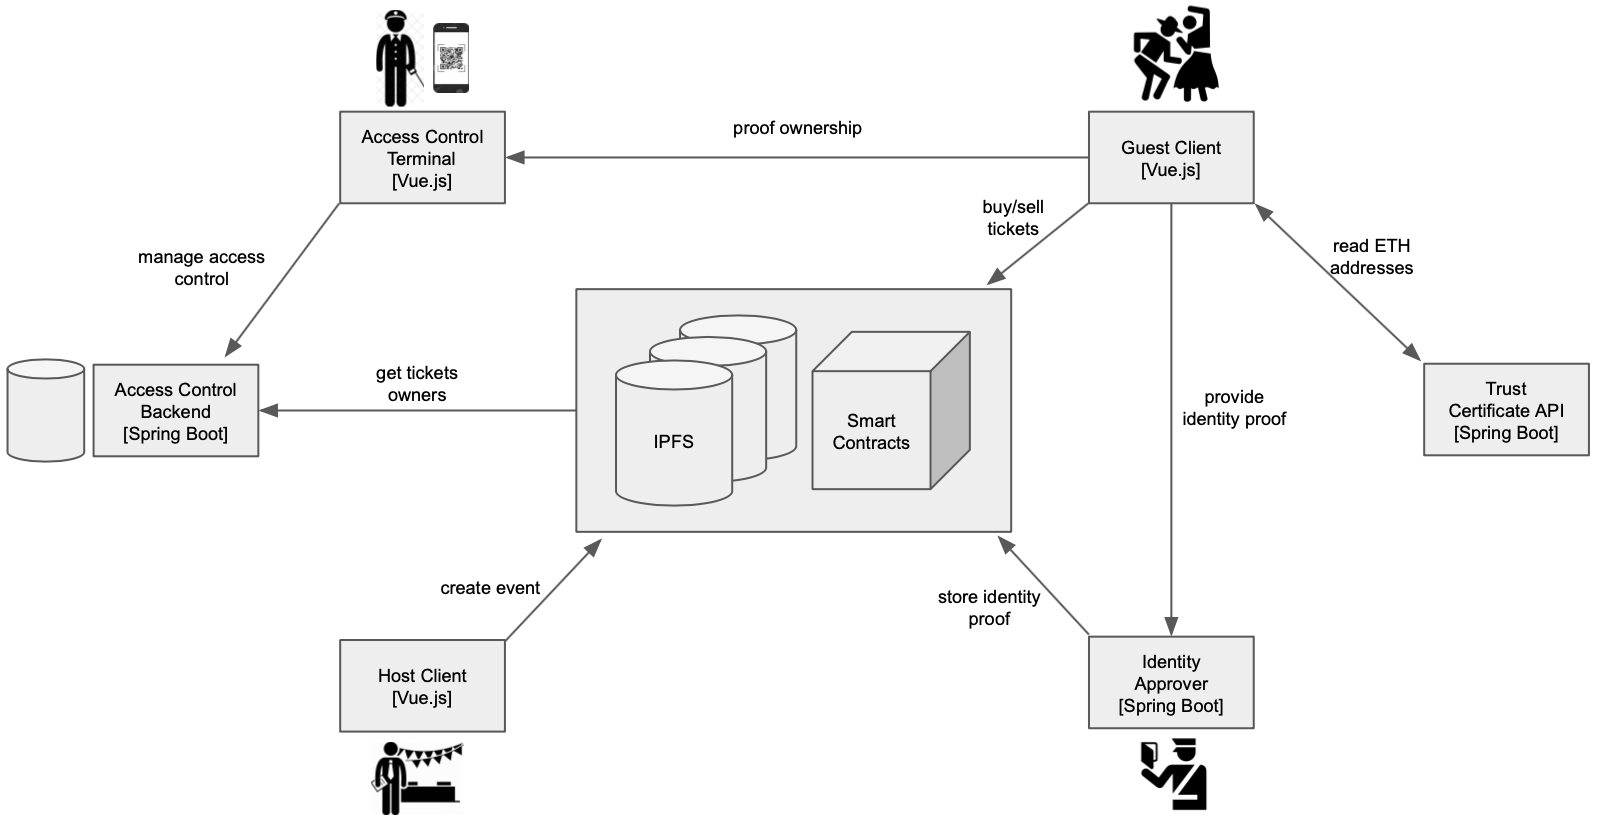
\includegraphics[width=16cm]{figures/architecutal-overview.png}
    \caption{Architectural overview of services}
    \label{fig:architecutral-overview}
\end{figure}


\section{Interactions}
This section covers the interactions between the different actors and the applications. Each Subsection will introduce an interaction in more detail.

\subsection{Buy a Ticket}
Figure \ref{fig:buyticket-sequence-diagram} shows the process, when a guest buys a ticket. Hereby, the guest interacts with the guest-client to buy a ticket. The client then sends the requests to buy a ticket to the event SC. The contract updates the owner of the bought ticket and locks the price in ETH until the event has passed. After the event, the host can request to receive the now unlocked ETH from SC to initiate the payment. This step is necessary, since a SC cannot initiate a transaction itself.
\begin{figure}[H]
    \centering
    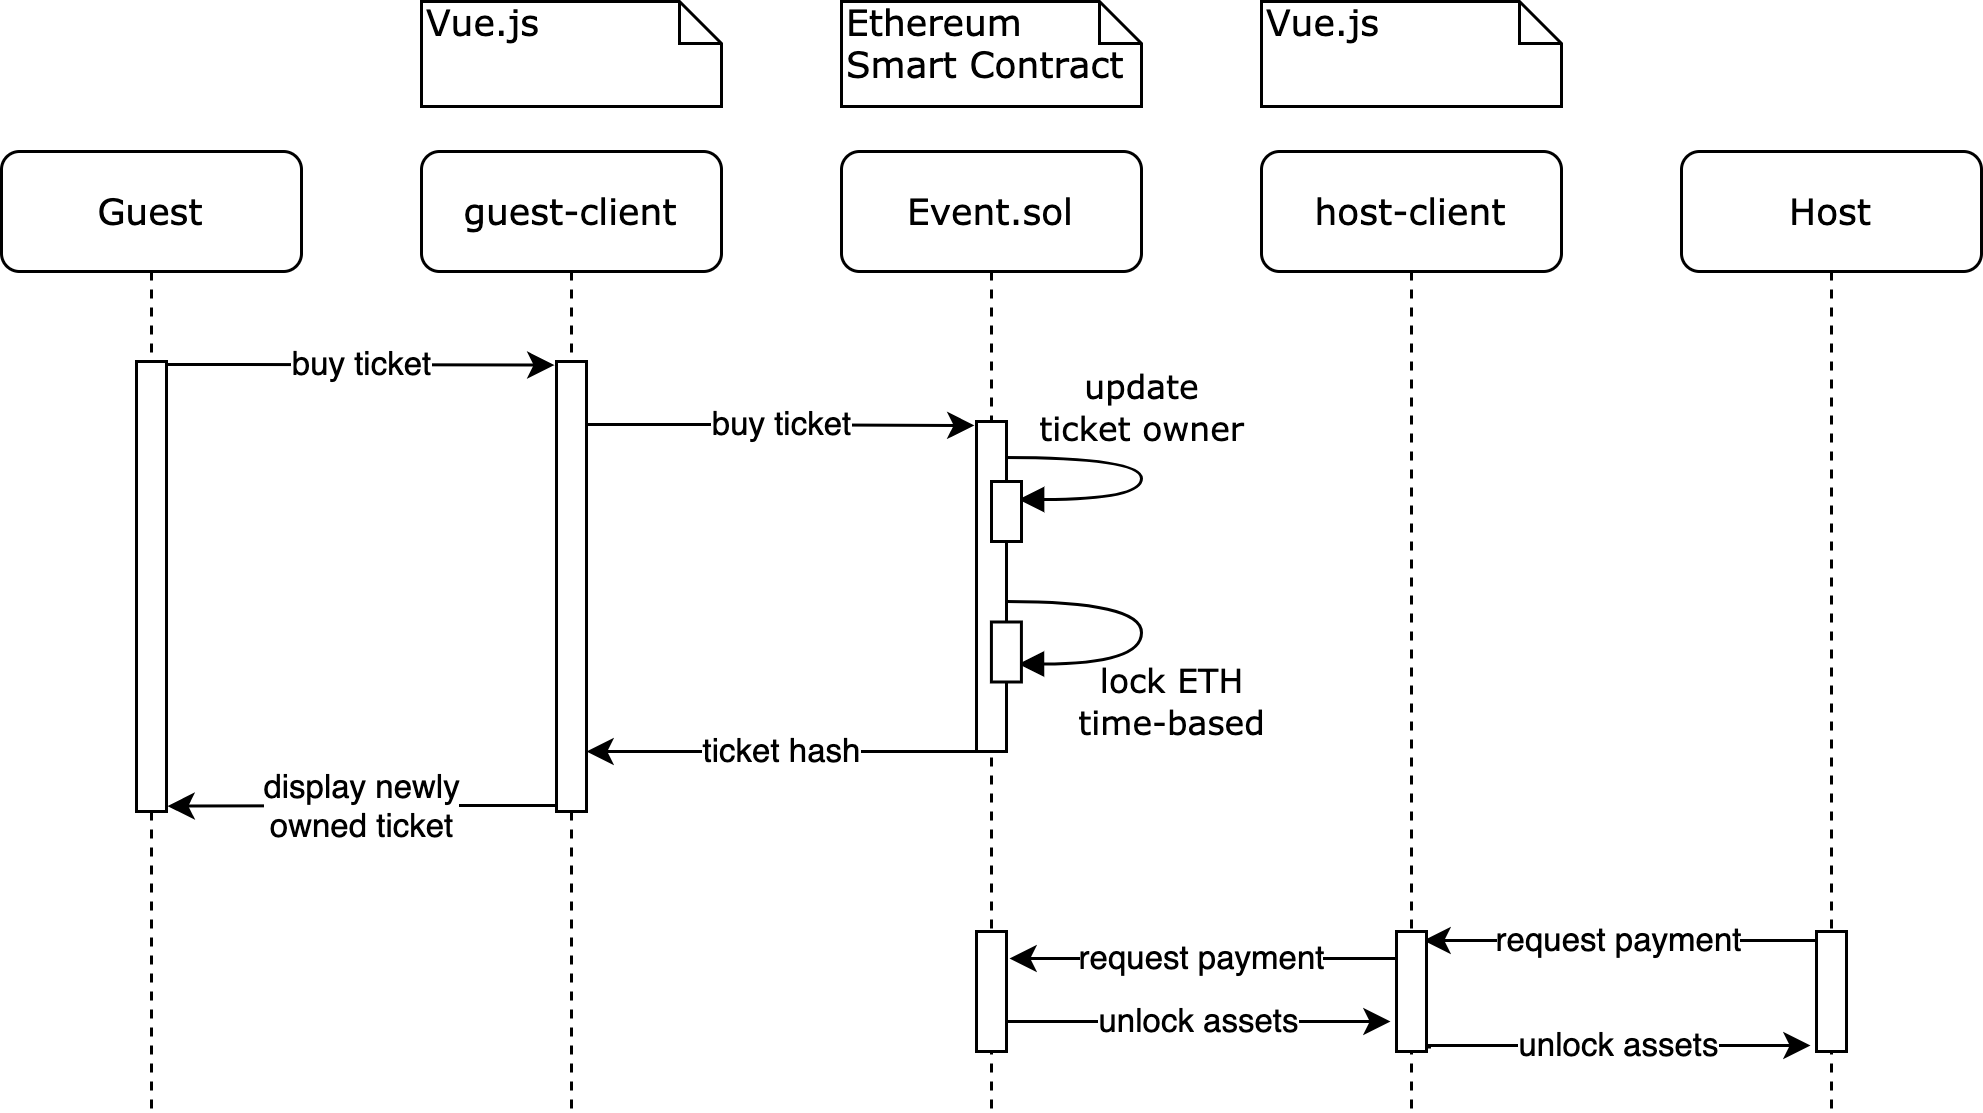
\includegraphics[width=16cm]{design/diagrams/BuyTicket.png}
    \caption{Ticket Sale Sequence Diagram}
    \label{fig:buyticket-sequence-diagram}
\end{figure}

\subsection{Presale}
The sequence diagram in Figure \ref{fig:presale-seuquence-diagram} illustrates how a guest can participate in a ticket presale. When registering for the presale, the ticket price is locked in the SC. The user has the option to opt-out at any time and get the locked ETH back. The event host decides when the presale ends. After this defined end time, the Event SC uses a source of randomness to determine the winners of the presale (see section\ref{section:imp:presale}). If a guest is part of the winners, he can mint his ticket. If not, the guest can claim the spent ETH back.

\begin{figure}[H]
    \centering
    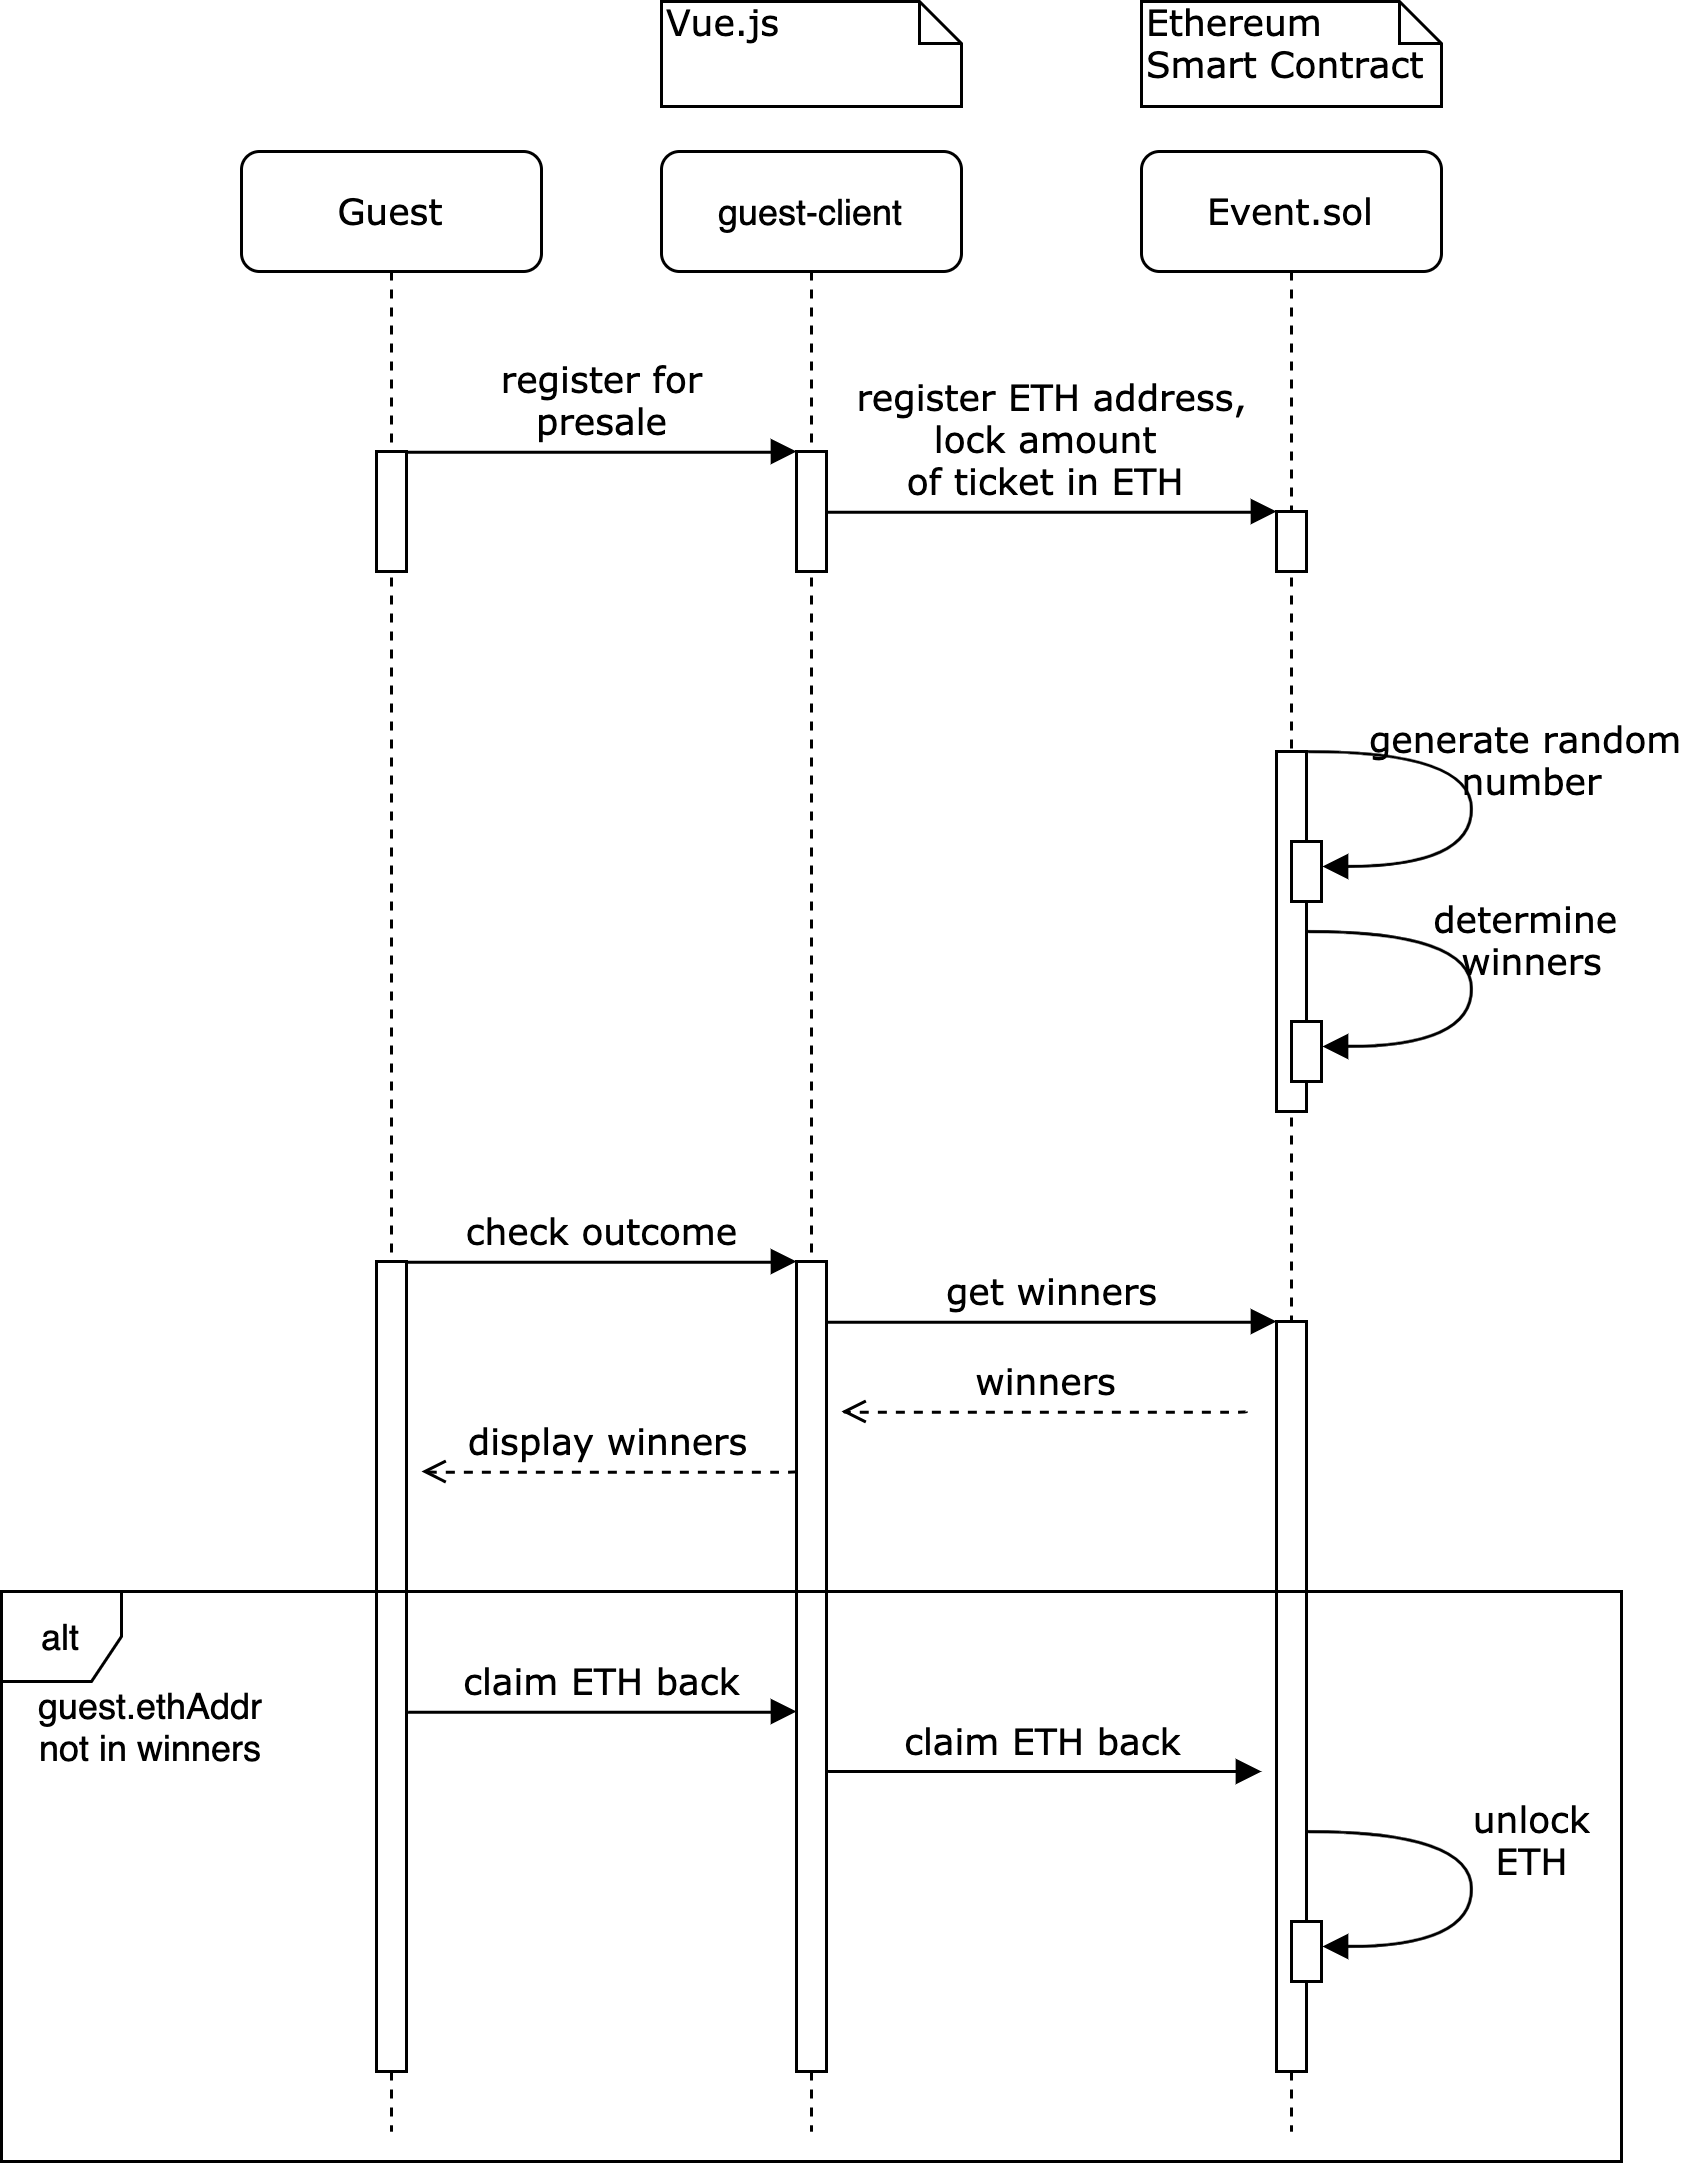
\includegraphics[width=14cm]{design/diagrams/presale.png}
    \caption{Presale Sequence Diagram}
    \label{fig:presale-seuquence-diagram}
\end{figure}

\subsection{Buy a Ticket from an Affiliate Link}
To broaden an event's visibility, a host may want to hire affiliates to promote their event. To do so, the host can register affiliates on the event SC, so that the affiliate can distribute a link containing his Ethereum address as query segment. The buying process is the same as in Figure \ref{fig:buyticket-sequence-diagram}. However, the affiliate's address is also forwarded to the SC and is linked to the bought ticket as well. After the event, when the ticket prices in ETH are unlocked, the affiliate can request to receive the award from each ticket that was sold holding his address as affiliate.
\begin{figure}[H]
    \centering
    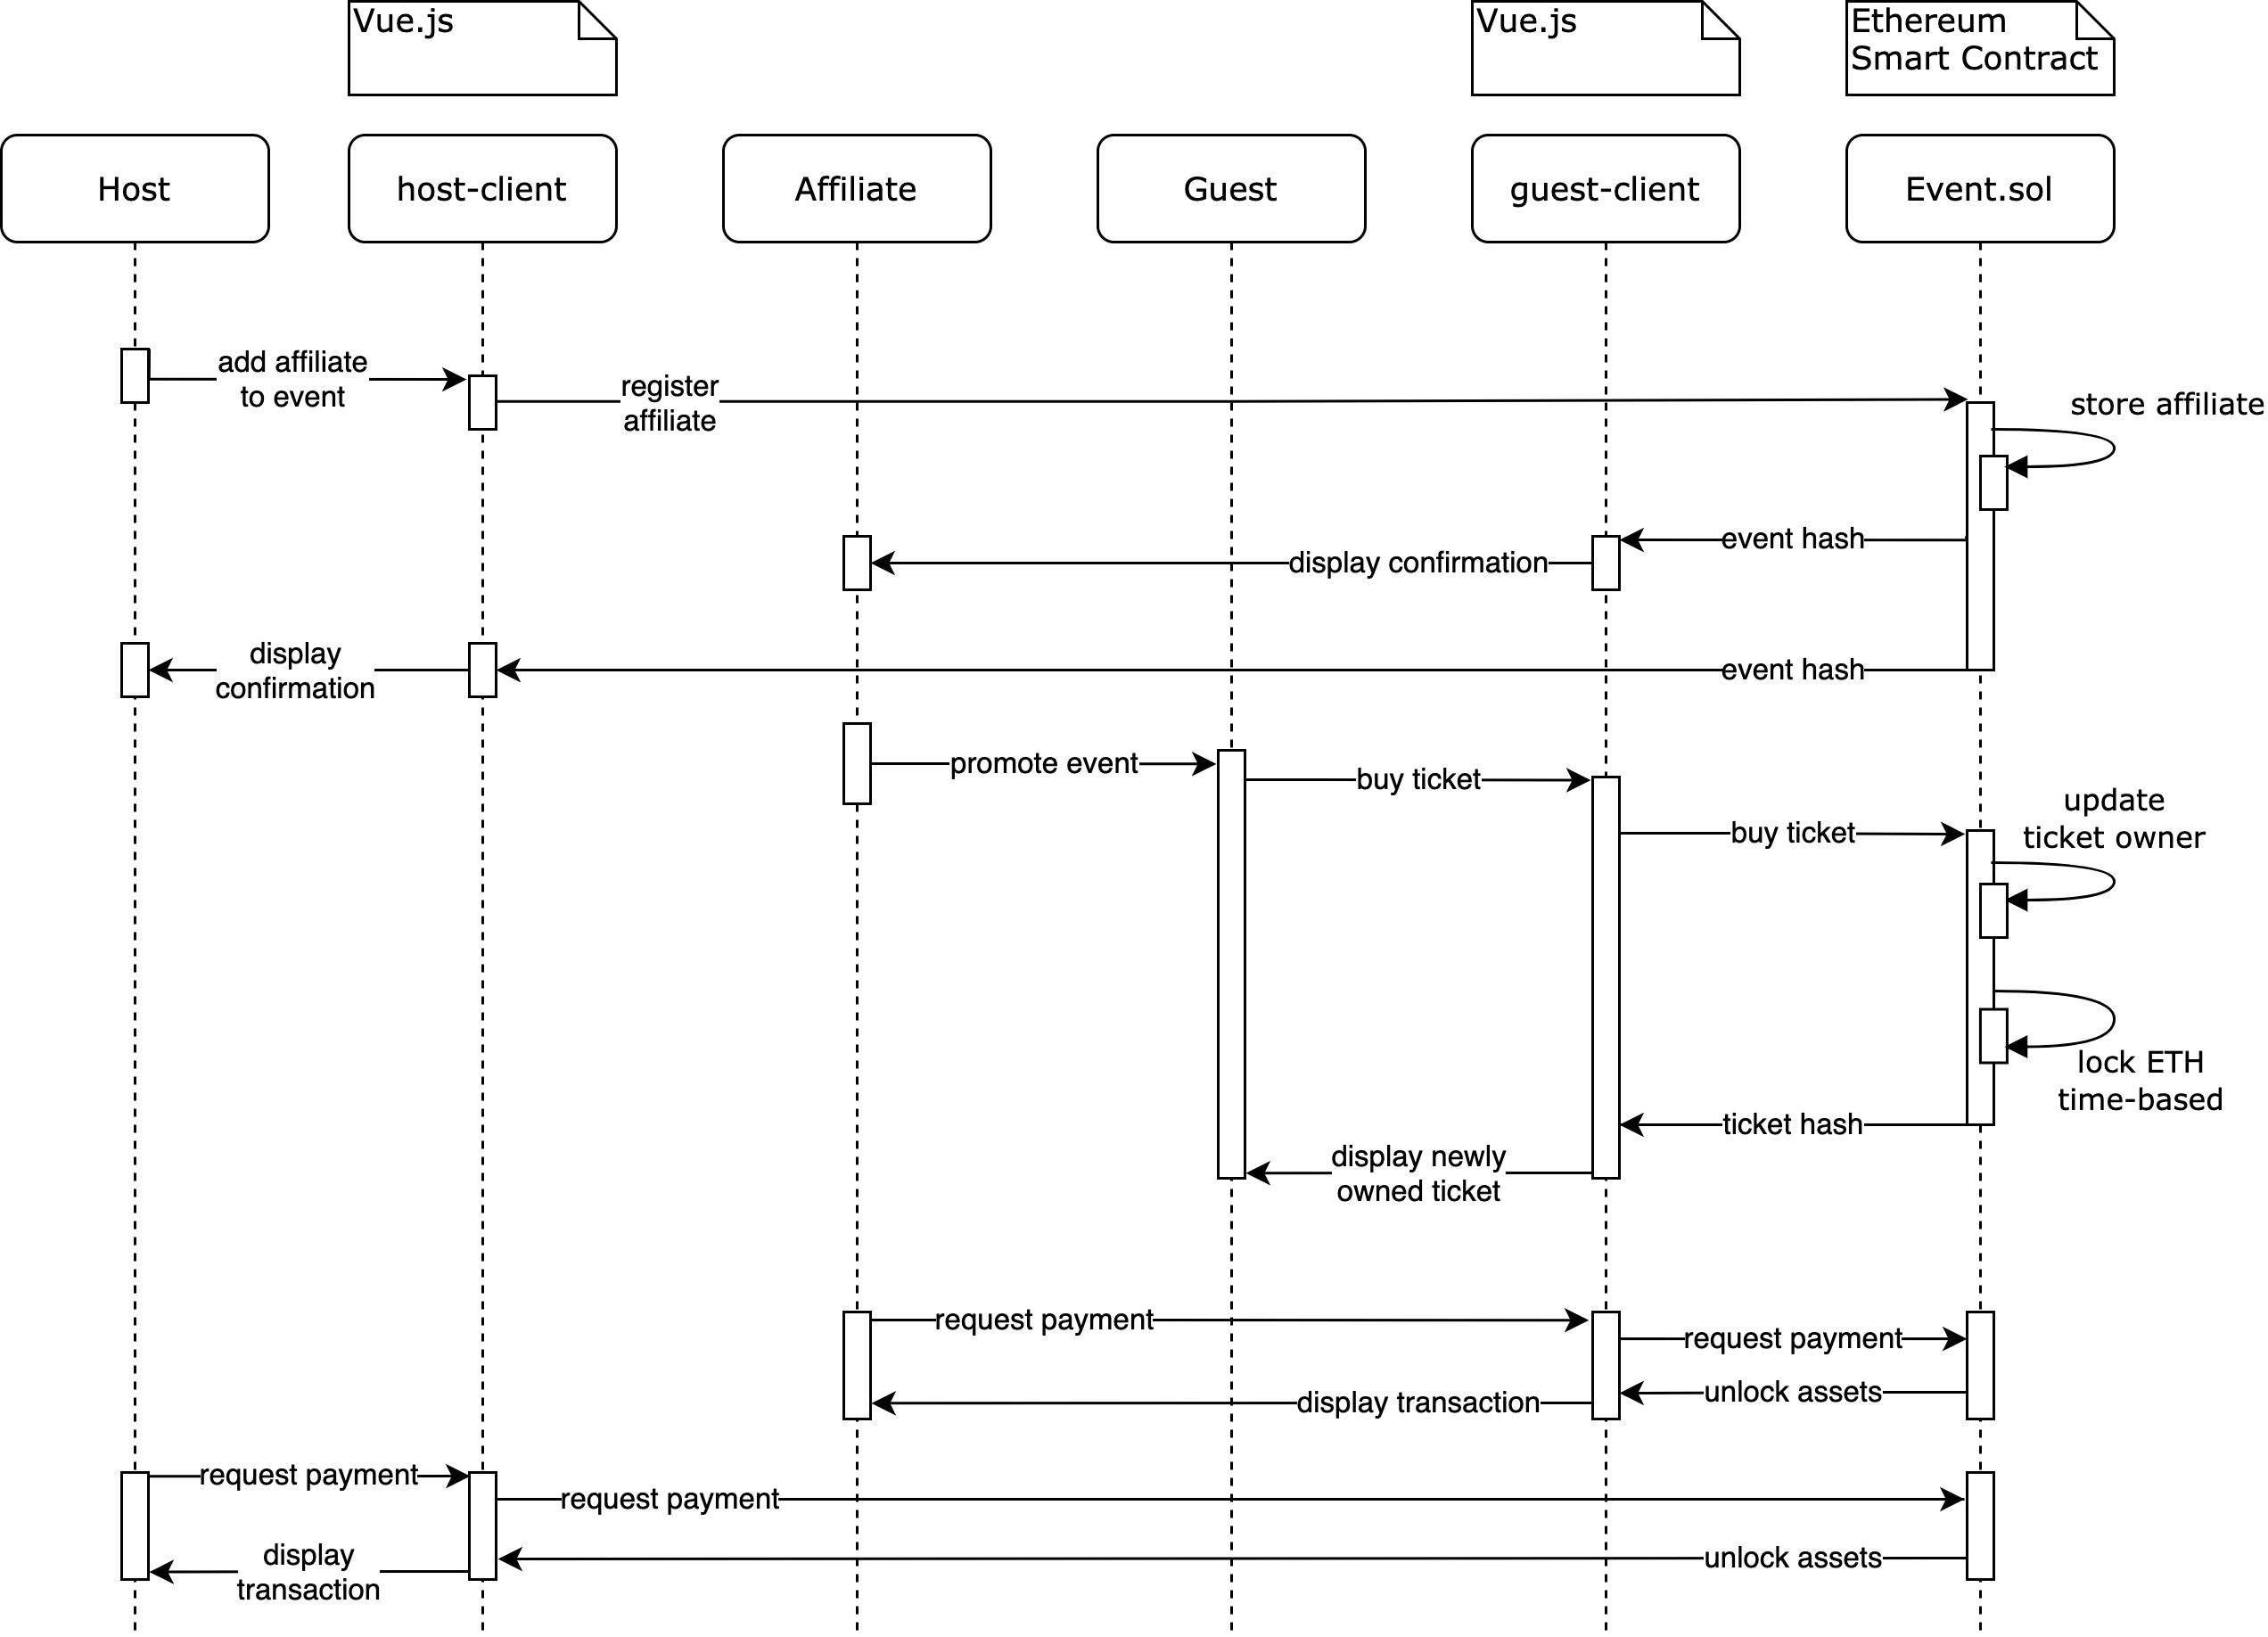
\includegraphics[width=16cm]{design/diagrams/BuyTicketFromAffiliateLink.png}
    \caption{Ticket Sale from Affiliate Link Sequence Diagram}
    \label{fig:buyticket-from-affiliate-diagram}
\end{figure}

\subsection{Identity Registration}
In Switzerland, to get a new phone number, you have to provide your passport details. Therefore a scalper cannot go through the process of approving his identity multiple times. The sequence diagram in Figure \ref{fig:identity-registration-airbnb} illustrates how a guest can prove his ownership of his phone number. To do so, the guest uses the \textit{guest-client} application to register an identity verification request. This request will be forwarded to the \textit{identity-approver} application. The identity approver is a trusted entity that checks if a user is in control of a certain Ethereum address, phone number, etc. In this scenario the user proofs his ownership of a phone number.  The idea of the identity approver is to store the uniqueness characteristic of that phone number and link it to a Ethereum address without the need of creating another KYC process. 

The identity approver generates a random sequence and sends it back to the identity the guest wants to proof ownership of. The guest receives the random sequence and enters it into the guest-client. The guest is then asked to sign the random sequence using his Ethereum address. The \textit{identity-approver} checks the signature for its validity. If this check completes successfully, a proof is generated.

Important to note is that the \textit{identity-approver} is a trusted entity. However, the goal is to build an application that does not rely on a single trusted entity. Thus, a system is envisioned where an event host can select from different identity approver and providers. It should even be possible that an event host can also act as the identity provider and approver. This would make sense for a large event company that want to make sure that no fraud is made by third parties. 

\begin{figure}[H]
    \centering
    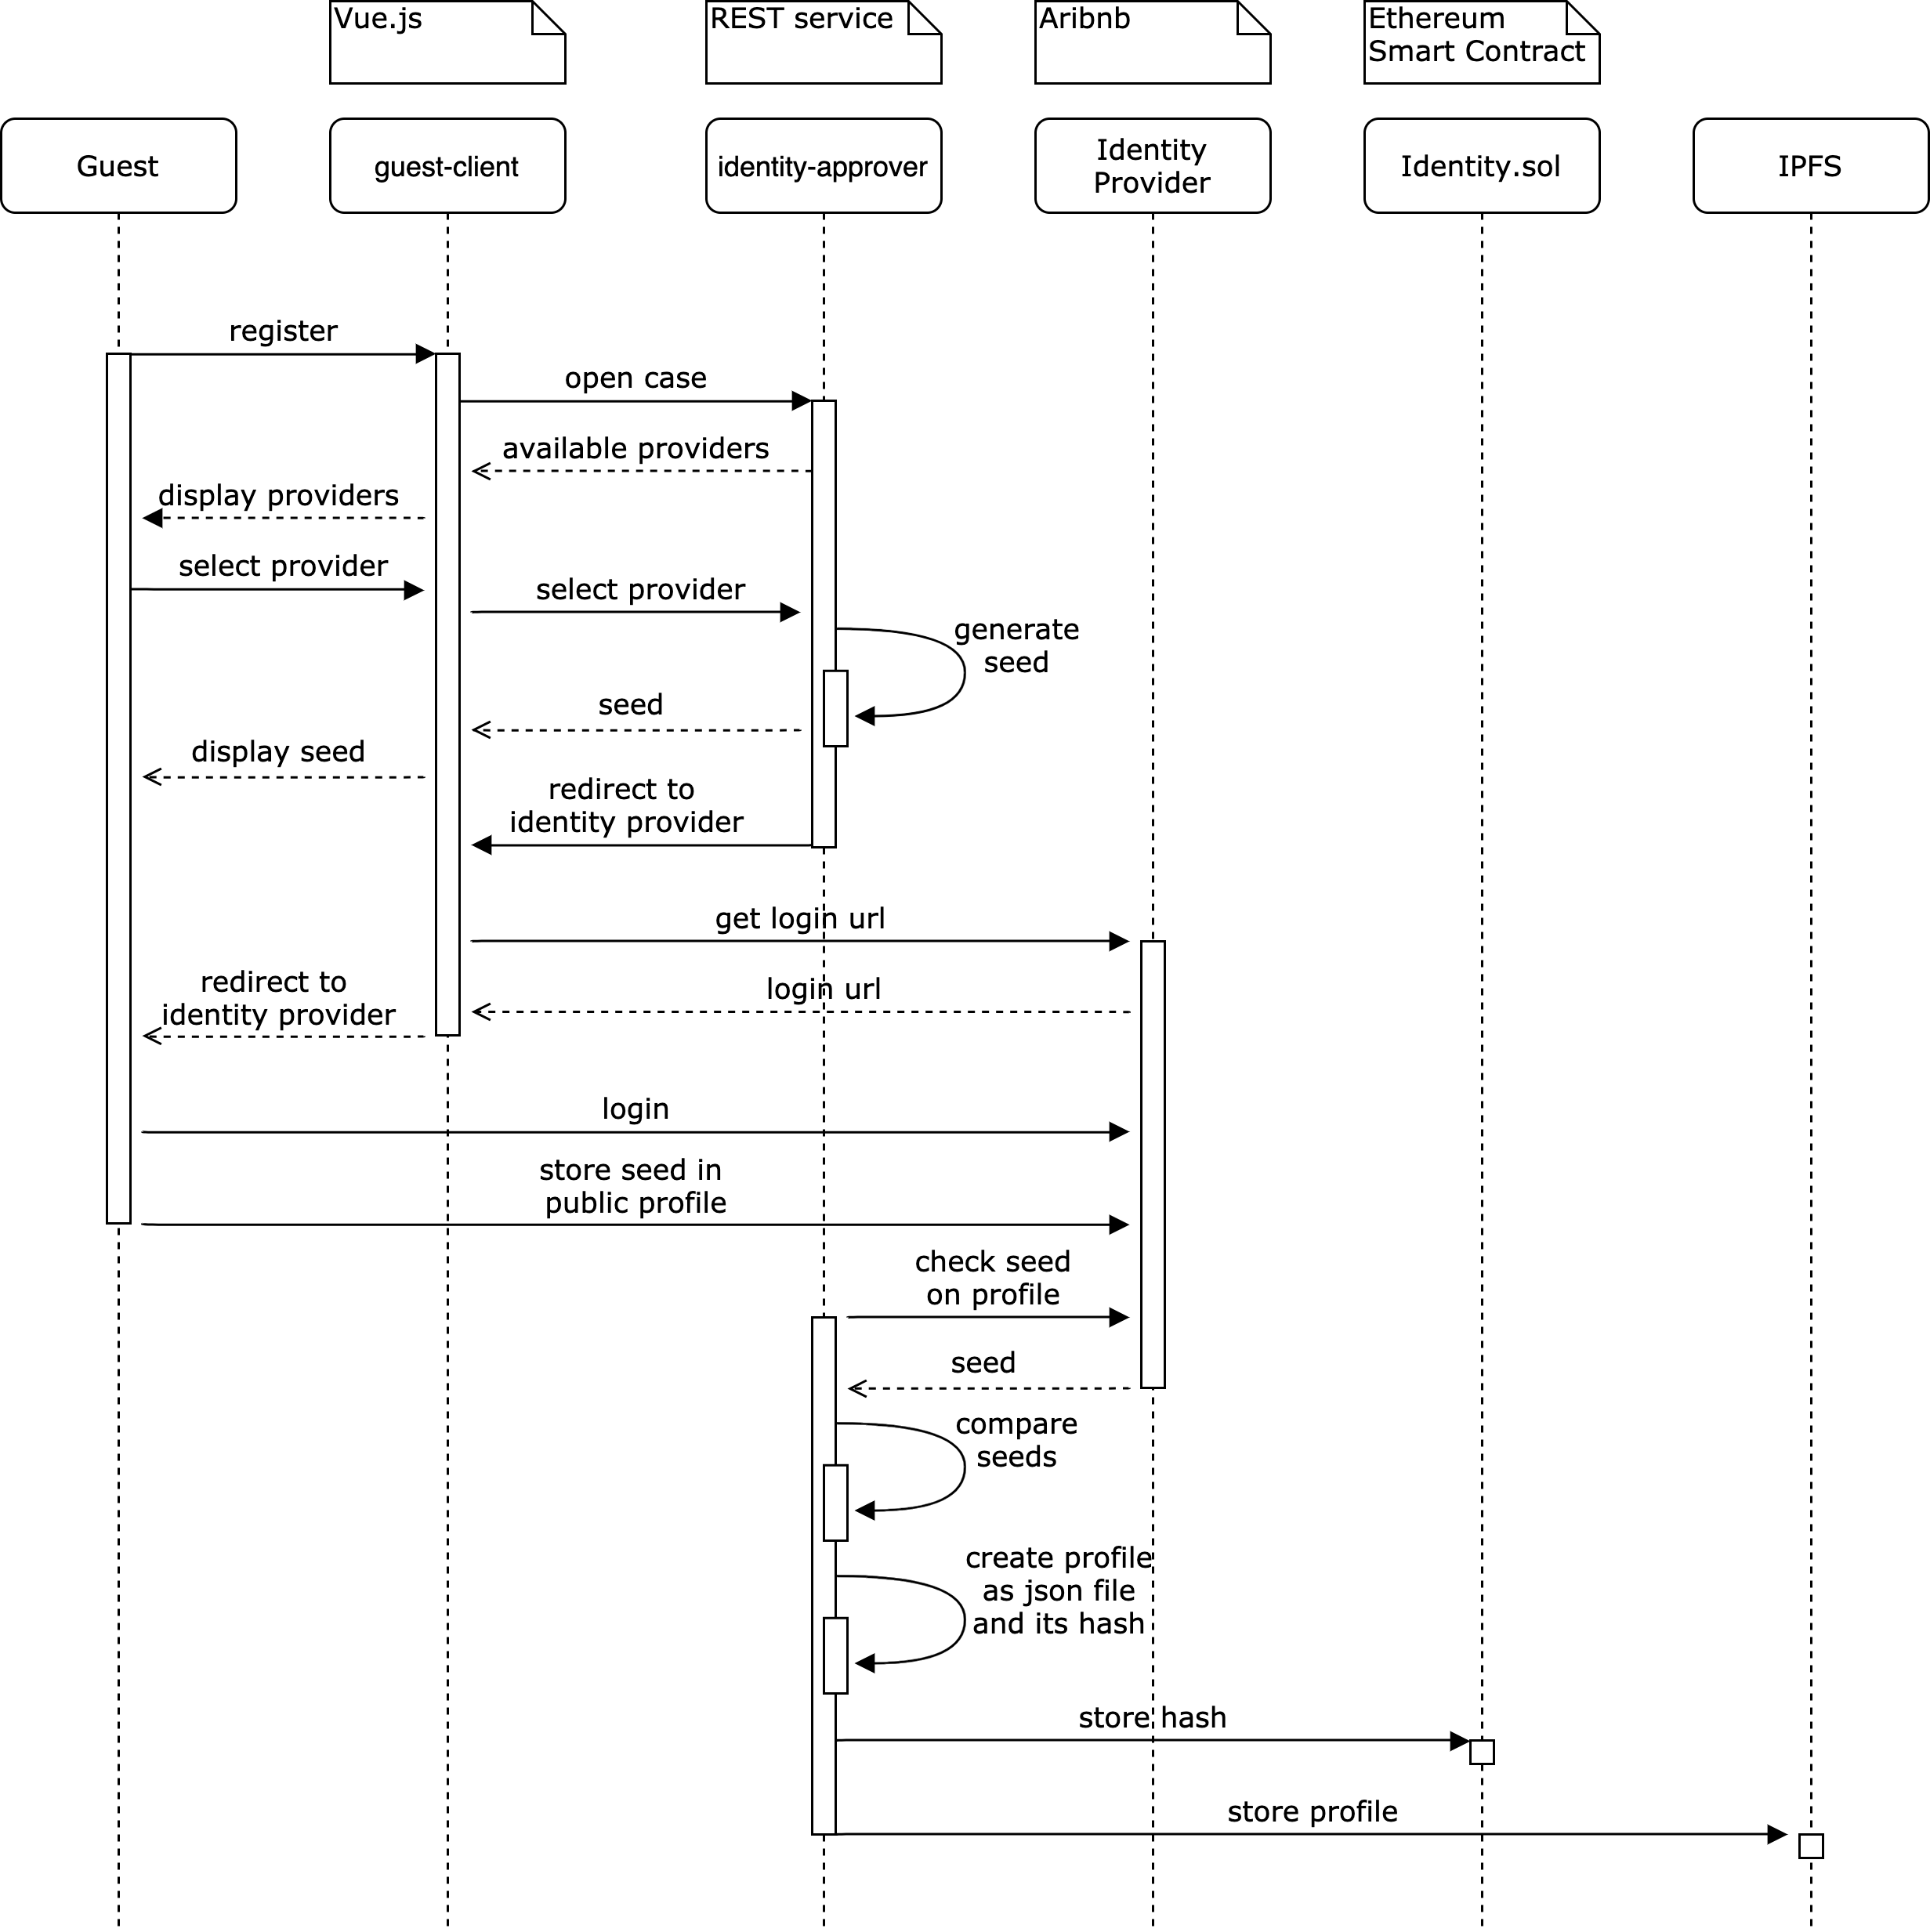
\includegraphics[width=16cm]{design/diagrams/identy-registration-airbnb.png}
    \caption{Identity Registration Phone number}
    \label{fig:identity-registration-airbnb}
\end{figure}

\subsection{Resell Ticket}
The guest logs into his account. The guest-client the gets all the Tickets owned by the guest, that are still valid. It then retrieves the ticket metadata form the IPFS storage. After the metadata has been retrieved, the guest gets shown the ticked owned by him. the guest then chooses the ticket he does no longer want to have and therefore selects the option to sell his ticket in the guest-client. This lists the ticket on the aftermarket. Whenever the ticket is bought by another guest, the money used to buy the ticket is directly transferred to the wallet of the seller of the ticket. When the guest checks his balance again, he will see the added funds.

This process is illustrated in the following sequence diagram.

\begin{figure}[H]
    \centering
    \includegraphics[width=16cm]{design/diagrams/Resell Ticket.png}
    \caption{Resell ticket}
    \label{fig:Resell-ticket}
\end{figure}

 


\subsection{Buy Ticket From Reseller}
\begin{figure}[H]
    \centering
    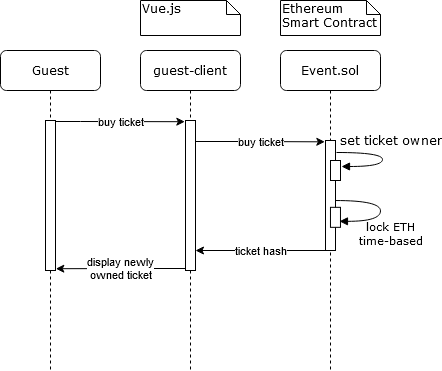
\includegraphics[width=12cm]{design/diagrams/BuyTicketFromResell.png}
    \caption{Buy Ticker from reseller}
    \label{fig:buyFromResell}
\end{figure}
The process of buying a ticket from the resell market looks exactly the same as buying directly from the host directly from the customers point-of-view, as depicted in \ref{fig:buyFromResell}. The Guest first connects to his wallet through his private key on the guest web application. Then he selects the event he is interested in and chooses to buy a ticket, which invokes the corresponding SC. Exactly as seen in \ref{fig:buyticket-sequence-diagram}, the SC locks the price of the ticket until the event has passed and returns the ticket hash to the guest web application, where it is displayed to the guest.

\subsection{Access Control}\label{subsection:access-control}

\begin{figure}[H]
    \centering
    \includegraphics[width=16cm]{design/diagrams/AcessControl.png}
    \caption{Access Control Sequence Diagram}
    \label{fig:access-controll}
\end{figure}

As the guest wants to gain access to the event, he is confronted with the entrance control. As the ticket is linked to the Ethereum address of the guest, he just has to prove the ownership of the given Ethereum address. In order to do this, the guest has to provide a signature of a message. This signature together with the message and the guest's public address can then be verified which ultimately proves that the guest owns this Ethereum address.

For this process three components are necessary. First of all, access terminal web applications (see section \ref{design:access-terminal}) are intended to run on tablet at the venue. They are used to display messages to be signed, a backend is needed to handle the signatures and keeping track of the state of the terminals and an embedded camera feature in the guest client application is required to scan the information from the terminal, sign the message and sending the signature to the backend for verification.

%Access terminals are placed at the respective entrances to display messages to be signed. A backend spring application provides an API to register terminals, create new messages for signing, verify signatures and check whether a ticket of the guest actually exists and was not already used to enter the event. 

%Access Terminals (see Subsection \ref{design:access-terminal}) are placed at the respective entrances. These terminals have to be registered with a secret code stored in the backend. When a terminal is registered, it is allocated a unique random sequence, which is stored in the backend and in the terminal application.

The entrance control terminals (see Subsection \ref{design:access-terminal}) are registered at the backend. Every terminal gets its unique identifier. The terminal then requests a unique random sequence, which is stored with the corresponding terminal id in the backend. This random sequence is then displayed alongside the backend URL as a QR-code on the terminal. The guest reads the QR-Code and extracts the random sequence. He then proceeds to sign the sequence using his Ethereum address proofing his ownership. The signature, the Ethereum address, the number of tickets he wants to use and the random sequence are then sent to the backend. The backend then evaluates the validity of the signature. After that, it is checked, whether the random sequence exists and the block chain is queried, to check, whether the Ethereum address actually holds enough tickets. It is also checked, whether this ticket already entered the venue. When all these checks are successful, the terminal, specified by its id, is messaged to let the guest pass. At the same time, the Ethereum address and the corresponding ticket are added to the database, that tracks the area the ticket owner are in. This implementation also holds for changing from different areas in a venue, for example accessing the VIP are from the general area of the venue.


%\begin{figure}[H]
%    \centering
%    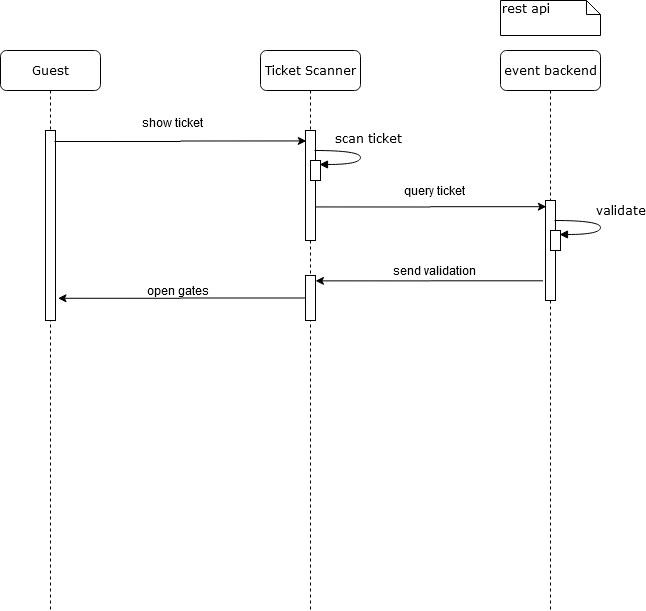
\includegraphics[width=14cm]{design/diagrams/entrance.png}
%    \caption{Entrance Control}
%    \label{fig:entranceControl}
%\end{figure}

%The sequence diagram in \ref{fig:entranceControl} depicts the process applied at the event gates for handling entrance control. The guest presents his ticket to the employee at the gate in form of a QR-code on his phone. The employee scans the code using the ticket scanner mobile application, which invokes a call to the rest API on the event backend, which contains a database with all tickets and the public keys of their respective owners. Once the Ticket Scanner application receives the confirmation from the server that the code is valid, the guest is granted access to the event.



% \subsection{Event Cancellation}
%This Section demonstrates how a guest can issue a report if an event was fraudulent or did not take place and the event host did not pay back the ticket price. 

%The sequence diagram in Figure \ref{fig:dispute-resolution-approved} shows how a guest rightfully reports a dispute and in Figure \ref{fig:dispute-resolution-rejected} the guest is not entitled to issue a dispute. 

%When the host creates an event, a fixed amount of ETH is locked as a deposit as well as a trusted third party is used to verify the guest's identification as explained in Figure \ref{fig:identity-registration-airbnb}. This party also acts as a dispute resolver. It is envisioned that this entity consists of multiple parties but for simplicity reasons it is shown as one ETH account. The deposit is locked until the challenge period is over. During the challenge period a guest can report fraudulent events.

%When the dispute resolver receives examination requests, they contact the event host for access proof. These proofs can only be generated by the ticket holders and contain the event id and the date of access. If the host can provide such requests, the tickets were used to enter the venue. The claim that the event was fraudulent is wrong and the host deposit will be unlocked for the host when the challenge period is over. 


%\begin{figure}[H]
%    \centering
%    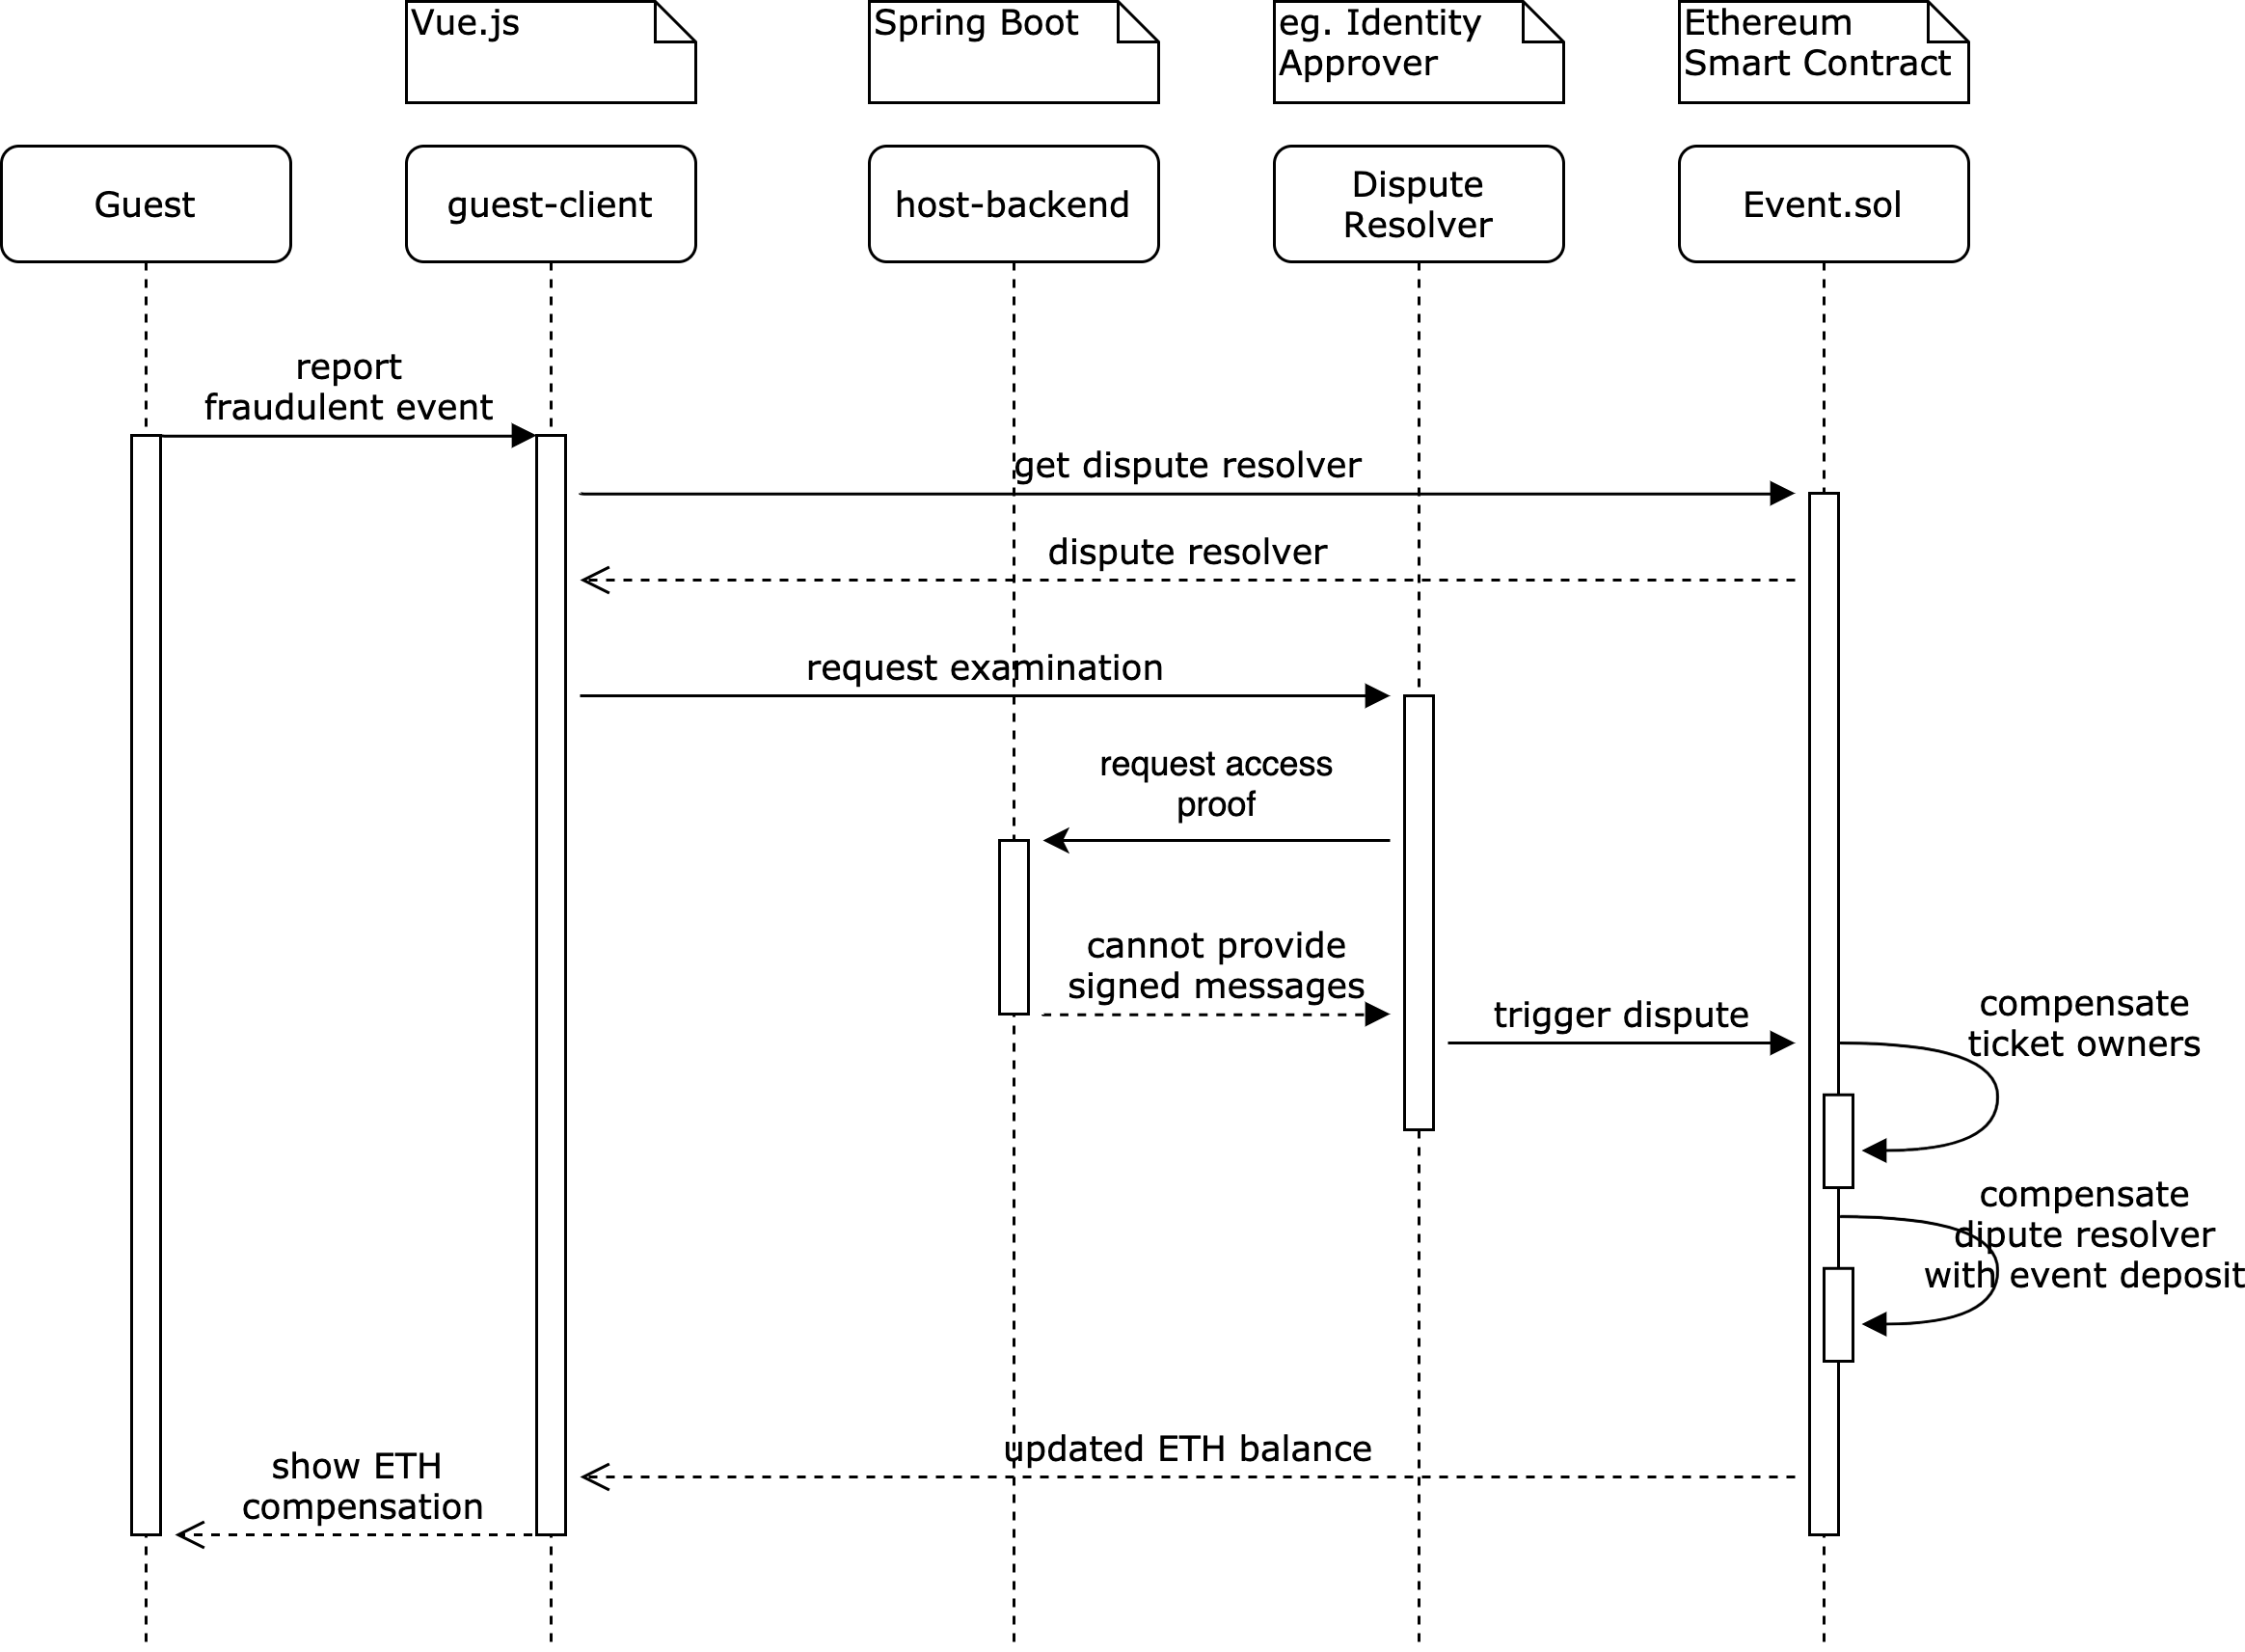
\includegraphics[width=16cm]{design/diagrams/dispute-resolution-approved.png}
%    \caption{Event Cancellation Approved}
%    \label{fig:dispute-resolution-approved}
%\end{figure}


%In the case where the event is fraudulent, the event host cannot provide signed proofs that tickets were used to enter the venue. The dispute resolver then calls the SC to send the locked ETH in the SC back to the ticket owners. Also the dispute resolver is compensated with the deposit that the event host initially had to deposit when the event was created. 

%\begin{figure}[H]
%    \centering
%    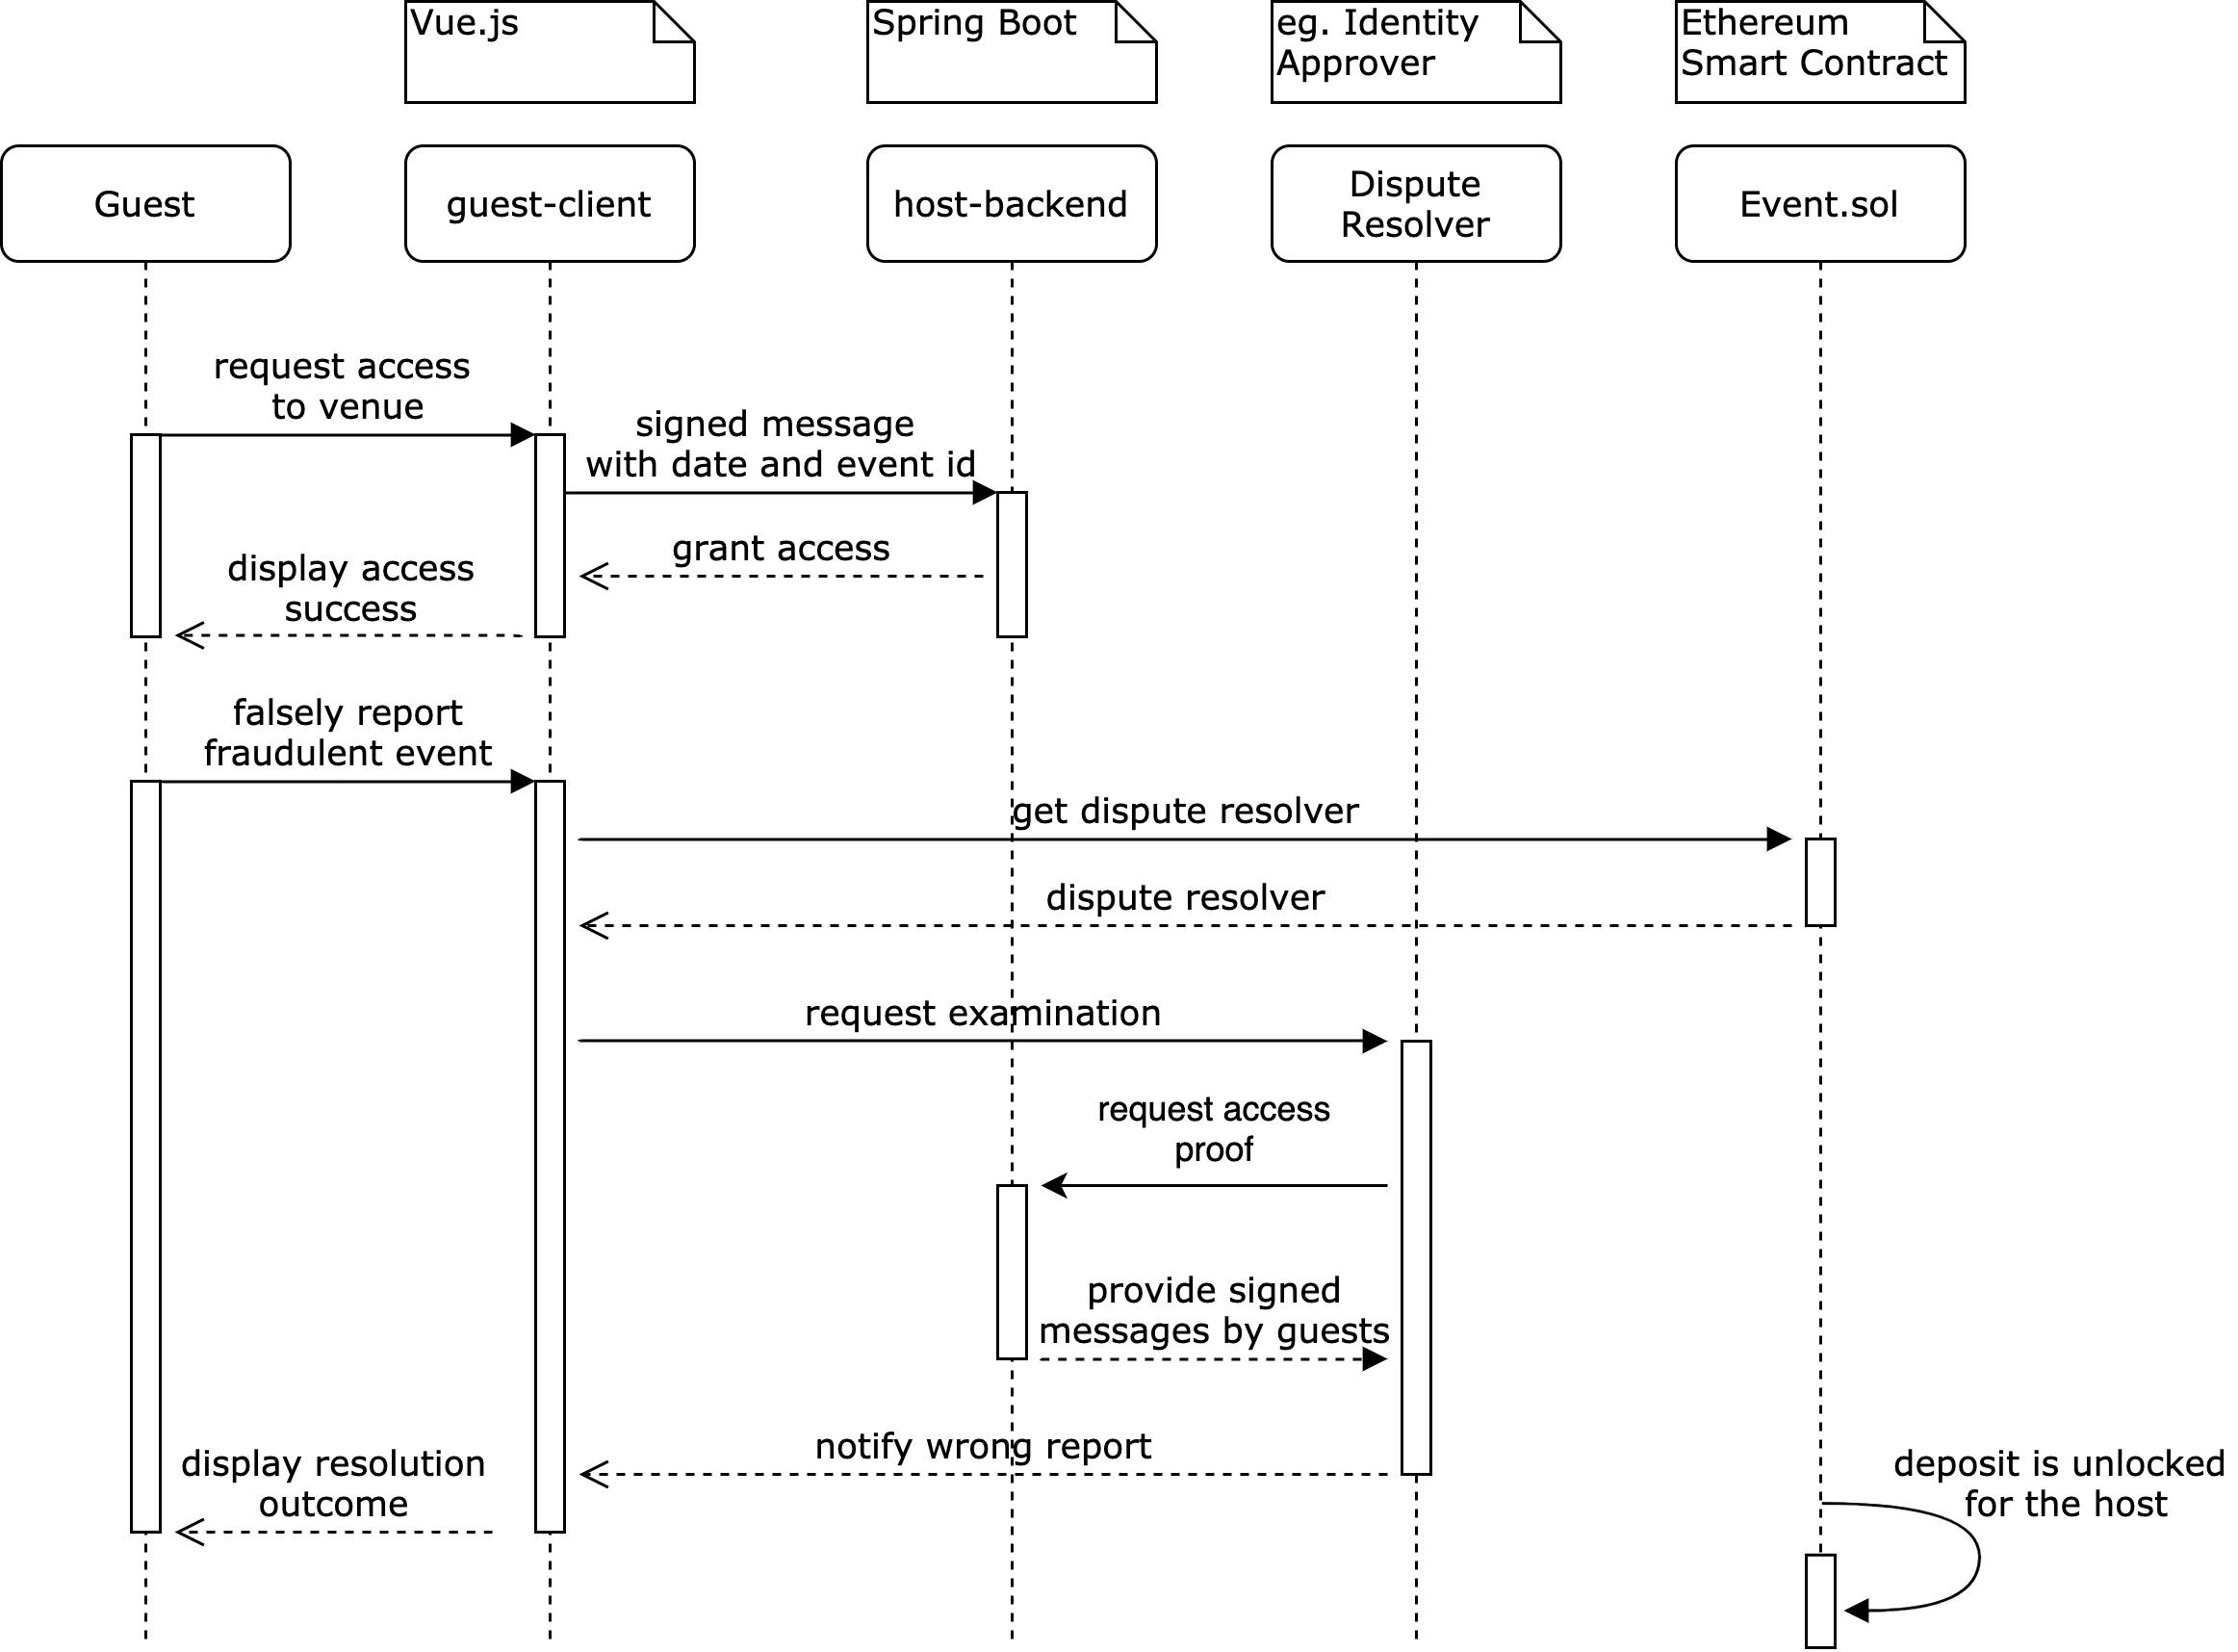
\includegraphics[width=16cm]{design/diagrams/dispute-resolution-rejected.png}
%    \caption{Event Cancellation Rejected}
%    \label{fig:dispute-resolution-rejected}
%\end{figure}
\section{Data Model}


\subsection{Smart Contract for Event Hosting}
The class diagram in Figure \ref{fig:event-data-model} illustrates how events are created and registered, tickets can be issued and distributed. Important to point out is that a presale only makes sense for fungible tickets. 
\begin{figure}[H]
    \centering
    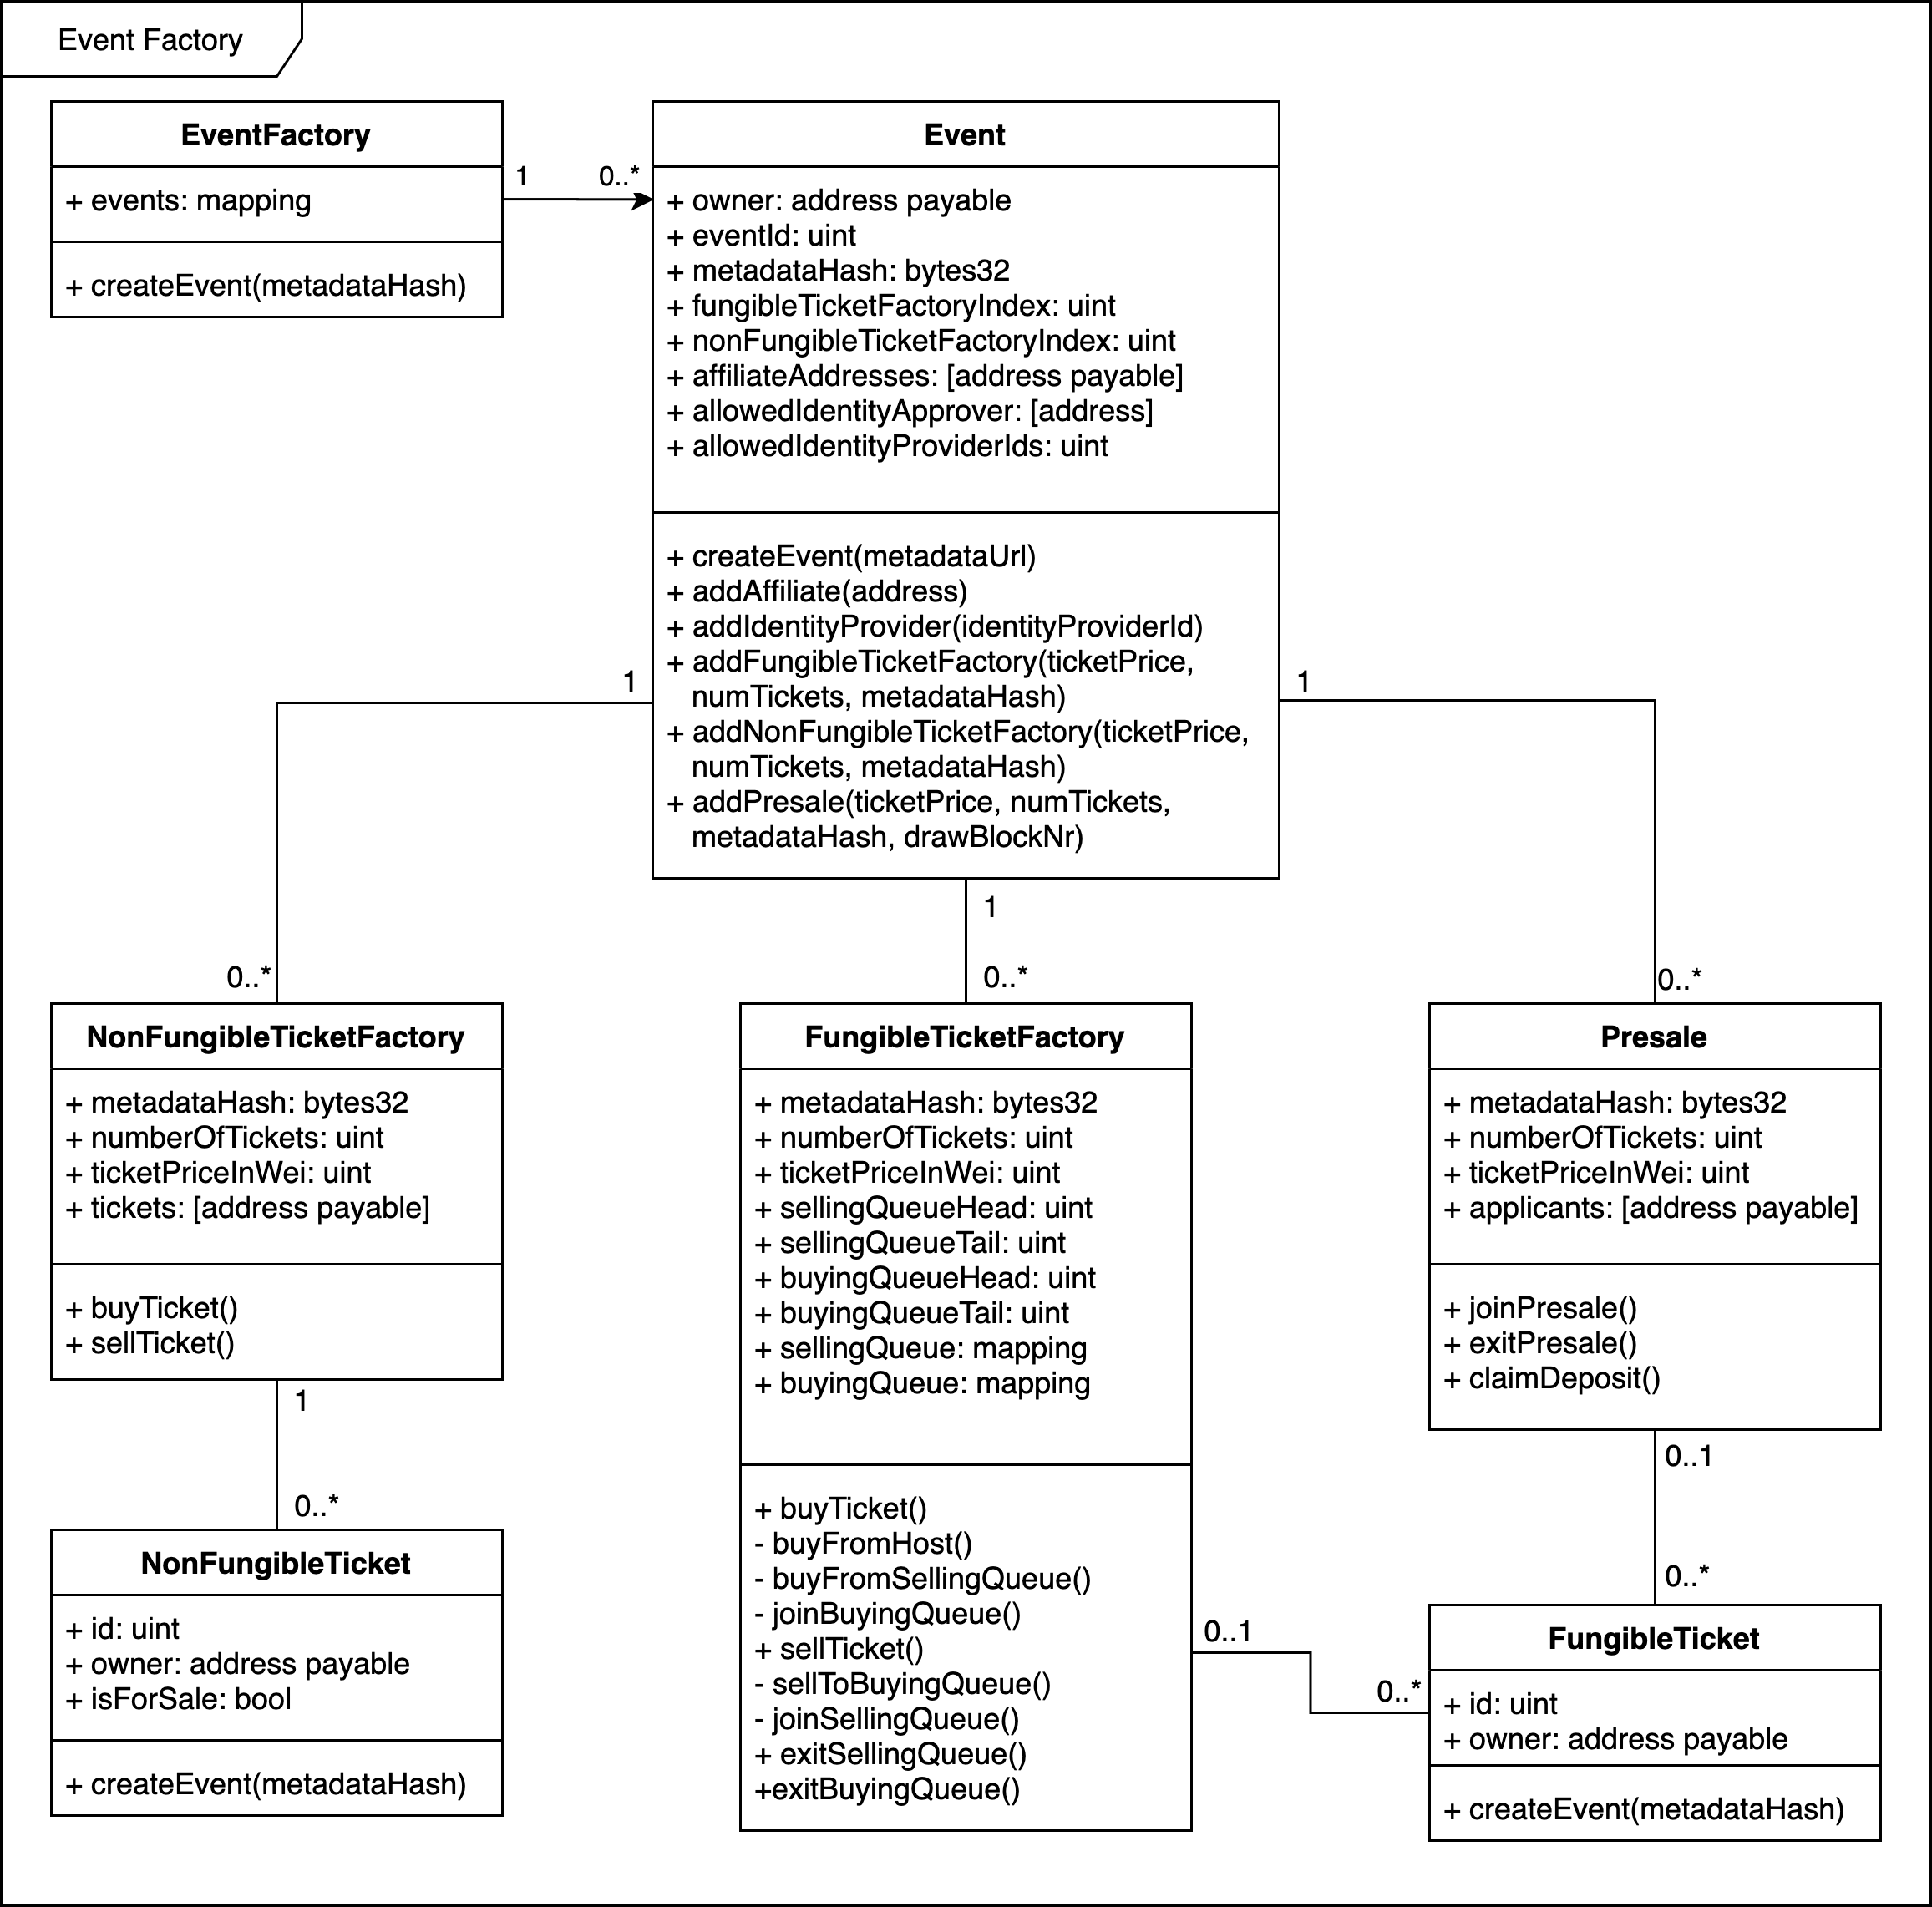
\includegraphics[width=16cm]{design/diagrams/event-factory-class-diagramm.png}
    \caption{Event Data Model}
    \label{fig:event-data-model}
\end{figure}

\subsection{Smart Contract for Identity Registration}

\subsection{RESTful Service for Identity Registration and Approval}
To interact with the identity approver, a Rest API as in Table \ref{tab:Identity-Reg-Rest-API} is used. The first step is to register an identity for approval. A secret will then be sent to this identity. In the next step, the identity is validated using the ETHadress and the secret received.

\begin{table}[H]
\caption{Identity Registration and Approval Rest API}
\label{tab:Identity-Reg-Rest-API}

\begin{tabular} { | m{0.3\textwidth} |m{0.1\textwidth}|m{0.2\textwidth}|m{0.2\textwidth} | }
\hline
Mapping & Type & Parameters & Return \\
\hline
  /addEmailIdentity & Post & eMail & boolean \\ 
\hline
/validateEmailIdentity & Post & eMail  & EmailIdentity \\ 
& &secret  & \\
& & signedSecret  & \\
& & ethAddress & \\
\hline
/addPhoneIdentity   & Post & phoneNr & boolean \\ 
\hline
/validatePhoneIdentity & Post & phoneNr & PhoneIdentity \\ 
& &secret  & \\
& & signedSecret  & \\
& & ethAddress & \\
\hline
\end{tabular}

\end{table}


\subsection{RESTful Service for Access Control}

\section{Technology Stack}\label{chapter:technology}

This section covers the technologies used within all separate parts of the ticketing platform.

\subsection{Client Web Applications}

The guest-client web application is the GUI provided for potential event guests interested in buying or selling tickets. The host-client web application is a tool for event organizers, which allows them to create events on the platform as well as to manage their events including the tickets.

Both web applications are built with Vue.js, a client-side JavaScript framework. Vue.js allows to integrate reactivity and application state management into websites and convinces through natively available modules for most essential parts of a modern web application.

In order to interact with the BC, the web3.js library is used. Web3.js provides wrapper functionality for data fetching from the BC and invoking remote SC calls. 
As mentioned in \ref{section:data-model}, the storage capabilities of SCs are highly limited. Thus, all event-related information (metadata) which is not critical for the core logic of the platform is stored externally. To keep the architecture as decentralized as possible, the metadata is stored on Inter Planetary File System (IPFS). IPFS is a peer-to-peer distributed file system, which is accessed from the guest-client application through a JavaScript API. To reduce the amount of remote calls to the BC and IPFS during application usage, the data is maintained within Vuex, a state management library provided for Vue.js. However, this storage is still in-memory and thus cleared with each application restart. Relying on solely runtime storage would require a full-fetch of all data on the BC with each application start, which introduces long loading times. In order to circumvent this, the clients use a second, persistent storage paradigm: The indexed Database (IDB). IDB is a schemaless datastore supported in most modern browsers which allows to store JSON-formatted data on the client device. The only caveat being that this storage is cleared when the user chooses to remove all browser data.

\subsubsection{Guest Client}

The goal of this application is to provide a user-friendly GUI for smartphones. Clients should be able to browse available events and their ticket categories. Users should also be able to connect their Ethereum wallet to the application to enable in-app ticket purchases and message signing. Vue.js provides an option to bundle a web application into a Progressive Web Application (PWA). PWAs can be installed as an application on most modern smartphones to be displayed in the application launcher. The aim is to emulate the experience of a native application as close as possible, while keeping the development perks of a web application such as rapid prototyping, expressive user interface (UI) modelling, and high availability of third-party libraries.

\subsection{Backend Applications}

The \textit{ID Approver} application is the application used to automatically verify the identity of a guest. The \textit{Access Control} application is used at the venue of the event to check whether a guest owns a ticket for the event.

Both backend applications are built using Spring Boot \footnote{\href{https://spring.io/projects/spring-boot}{https://spring.io/projects/spring-boot}} and are connected to a Structured Query Language (SQL) database to persist data. Spring Boot is used, since it allows to easily provide a REST API\footnote{\href{https://en.wikipedia.org/wiki/Representational_state_transfer}{https://en.wikipedia.org/wiki/Representational\_state\_transfer}} and also has a lot of support for 3rd party dependencies such as Twilio\footnote{\href{https://www.twilio.com/}{https://www.twilio.com/}} or Amazon Web Services\footnote{\href{https://aws.amazon.com/}{https://aws.amazon.com/}} (AWS).

To interact with the Ethereum BC, the Java library web3j\footnote{\href{https://docs.web3j.io/}{https://docs.web3j.io/}} is used. 
The application can connect to a local Ethereum node or use third party services such as infura\footnote{\href{https://infura.io/}{https://infura.io/}} to connect to the BC.
The application is built into a docker image and hosted on docker-hub\footnote{\href{https://hub.docker.com/}{https://hub.docker.com/}}. This allows anybody to just provide the required parameters for the used third party services in order to run the example implementation.  
Docker-compose\footnote{\href{https://docs.docker.com/compose/}{https://docs.docker.com/compose/}} is used to run the Spring Boot application in combination with a MySQL\footnote{\href{https://hub.docker.com/_/mysql}{https://hub.docker.com/\_/mysql}} docker image. This ensures easy deployment for anybody.



\subsection{Blockchain and Smart Contracts}
Ethereum is used as the BC application platform. SCs are scripts that run on each node in the Ethereum Virtual Machine (EVM) and enable the developer to store complex data structures and business logic in a distributed manner. 

The reason for choosing Ethereum was due to the broad range of developer tools auch as Truffle\footnote{\href{https://www.trufflesuite.com/}{https://www.trufflesuite.com/}} and Ganache\footnote{\href{https://www.trufflesuite.com/ganache}{https://www.trufflesuite.com/ganache}}. These tools allow the developer to run a local Ethereum BC with immediate block mining and deploy, test and evaluate the written SC. 





% author: Simon Bachmann

\section{Smart Contracts}\label{section:smart-contracts-design}

This section covers all the architectural decisions that affect the SC design. 

\subsection{Aftermarket}\label{section:aftermarket}
As explained in Section \ref{subsection:dex} there exist multiple types of DEXs. The design of each type of exchange underlies a trade-off between number of on-chain transactions (speed/network fees/user experience) and the degree of decentralization. The on-chain order book is decentralized but lacks in terms of speed and low gas fees. The off-chain order book and on-chain settlement results in less fees and higher throughput but requires third parties to broadcast the orders of all participants and not censor any user. Thus, it comes at the cost of decentralization. Liquidity pools suffer from slippage. Thus, executing multiple small orders results in a better exchange rate.

One of the goals of this project is to build a regulated but decentralized aftermarket and to prevent the emergence of a black market with unregulated prices. It must not be possible to find a seller on another platform and perform the ownership transfer through the regulated aftermarket. With the architecture of existing decentralized exchanges such an attack is possible. In this project it is referred as the black market attack and explained in more detail in Section \ref{subsection:black-market-attack}. 

This problem can be solved by using a queuing system for the aftermarket. The contract enforces a user to sell or buy a ticket from the head of the queue. In other words, a ticket is always sold to the person that created a buy order first. 

The aftermarket architecture consists of a \textit{buying queue} where users can queue up that are interested in buying a ticket and a \textit{selling queue} where people can queue up for selling their previously acquired tickets. Users are automatically matched if the opposite queue is not empty. The state of the system does not allow to have people in both queues at the same time. 

Figure \ref{fig:aftermarket-queue} illustrates how the queuing architecture works. The number below each person indicates how many ticket he is willing to buy/sell. A \textit{head pointer} is used in both queues to find the next buyer/seller in constant time. The \textit{tail pointer} is used to enqueue a new buyer/seller. However, it is possible that a person leaves the queue as indicated with the potential buyer at index 2. This user is no longer interested in buying a ticket.

\begin{figure}[H]
    \centering
    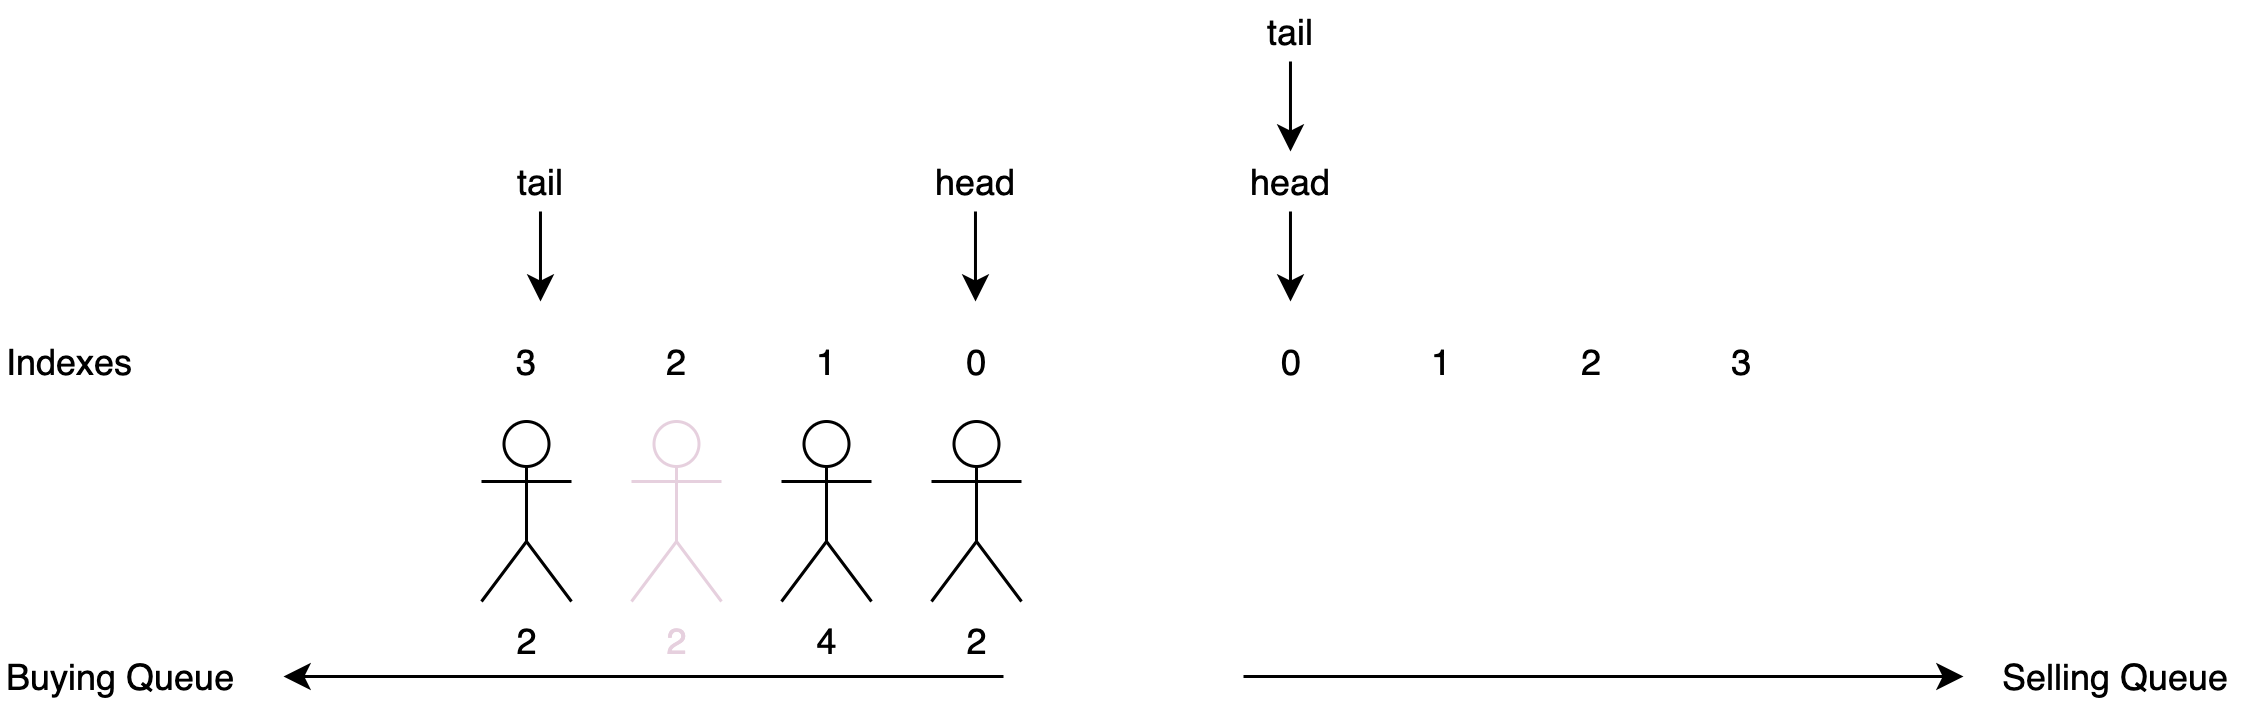
\includegraphics[width=16cm]{figures/aftermarket-queue.png}
    \caption{Aftermarket with buying and selling queue}
    \label{fig:aftermarket-queue}
\end{figure}

An important note to make is that an order might run into an \textit{out-of-gas exception}, if many consecutive buyers or sellers leave the queue because finding the head of the queue takes multiple loop iterations. In such a scenario, the users has to iterate over all the users that left the queue before finding a buyer/seller. 

This problem can be solved by adding function to the SC that reads how many people must be skipped before finding an actual buyer/seller. This must be a read-only function and does not cost any network fees. The result of read operation can be used to set an adequate network fee for the buy/sell order. 

\subsection{Dynamic Pricing}
To allow dynamic pricing below the original price, an architecture was designed to accomplish multiple buying and selling queues with fixed prices. The creator of an event can configure the aftermarket with an arbitrary number of queues. However, it is a trade-off between granular pricing and the possibility of allowing a black market to emerge. When configuring too many queues, it is possible to facilitate a trade between a buyer and seller from the black market. This can be achieved by selecting a pair of buying and selling queue which both are empty similar to the scenario explained in an open order book in Section \ref{section:aftermarket}. When configuring too little queues, the end user is restricted in setting the desired reselling price. 

The fixed prices are defined by using a percentage of the original prices and the granularity can be configured by the event owner. 

The following scenarios describe possible states of the aftermarket. Figure \ref{fig:aftermarket-high-demand} shows how multiple people queued up in the buying queues meaning that the demand for this type of ticket is high. A ticket owner can immediately sell his ticket to any person at the head of each queue. Of course to maximize profit, one should always choose the queue that offers the highest price.

\begin{figure}[H]
    \centering
    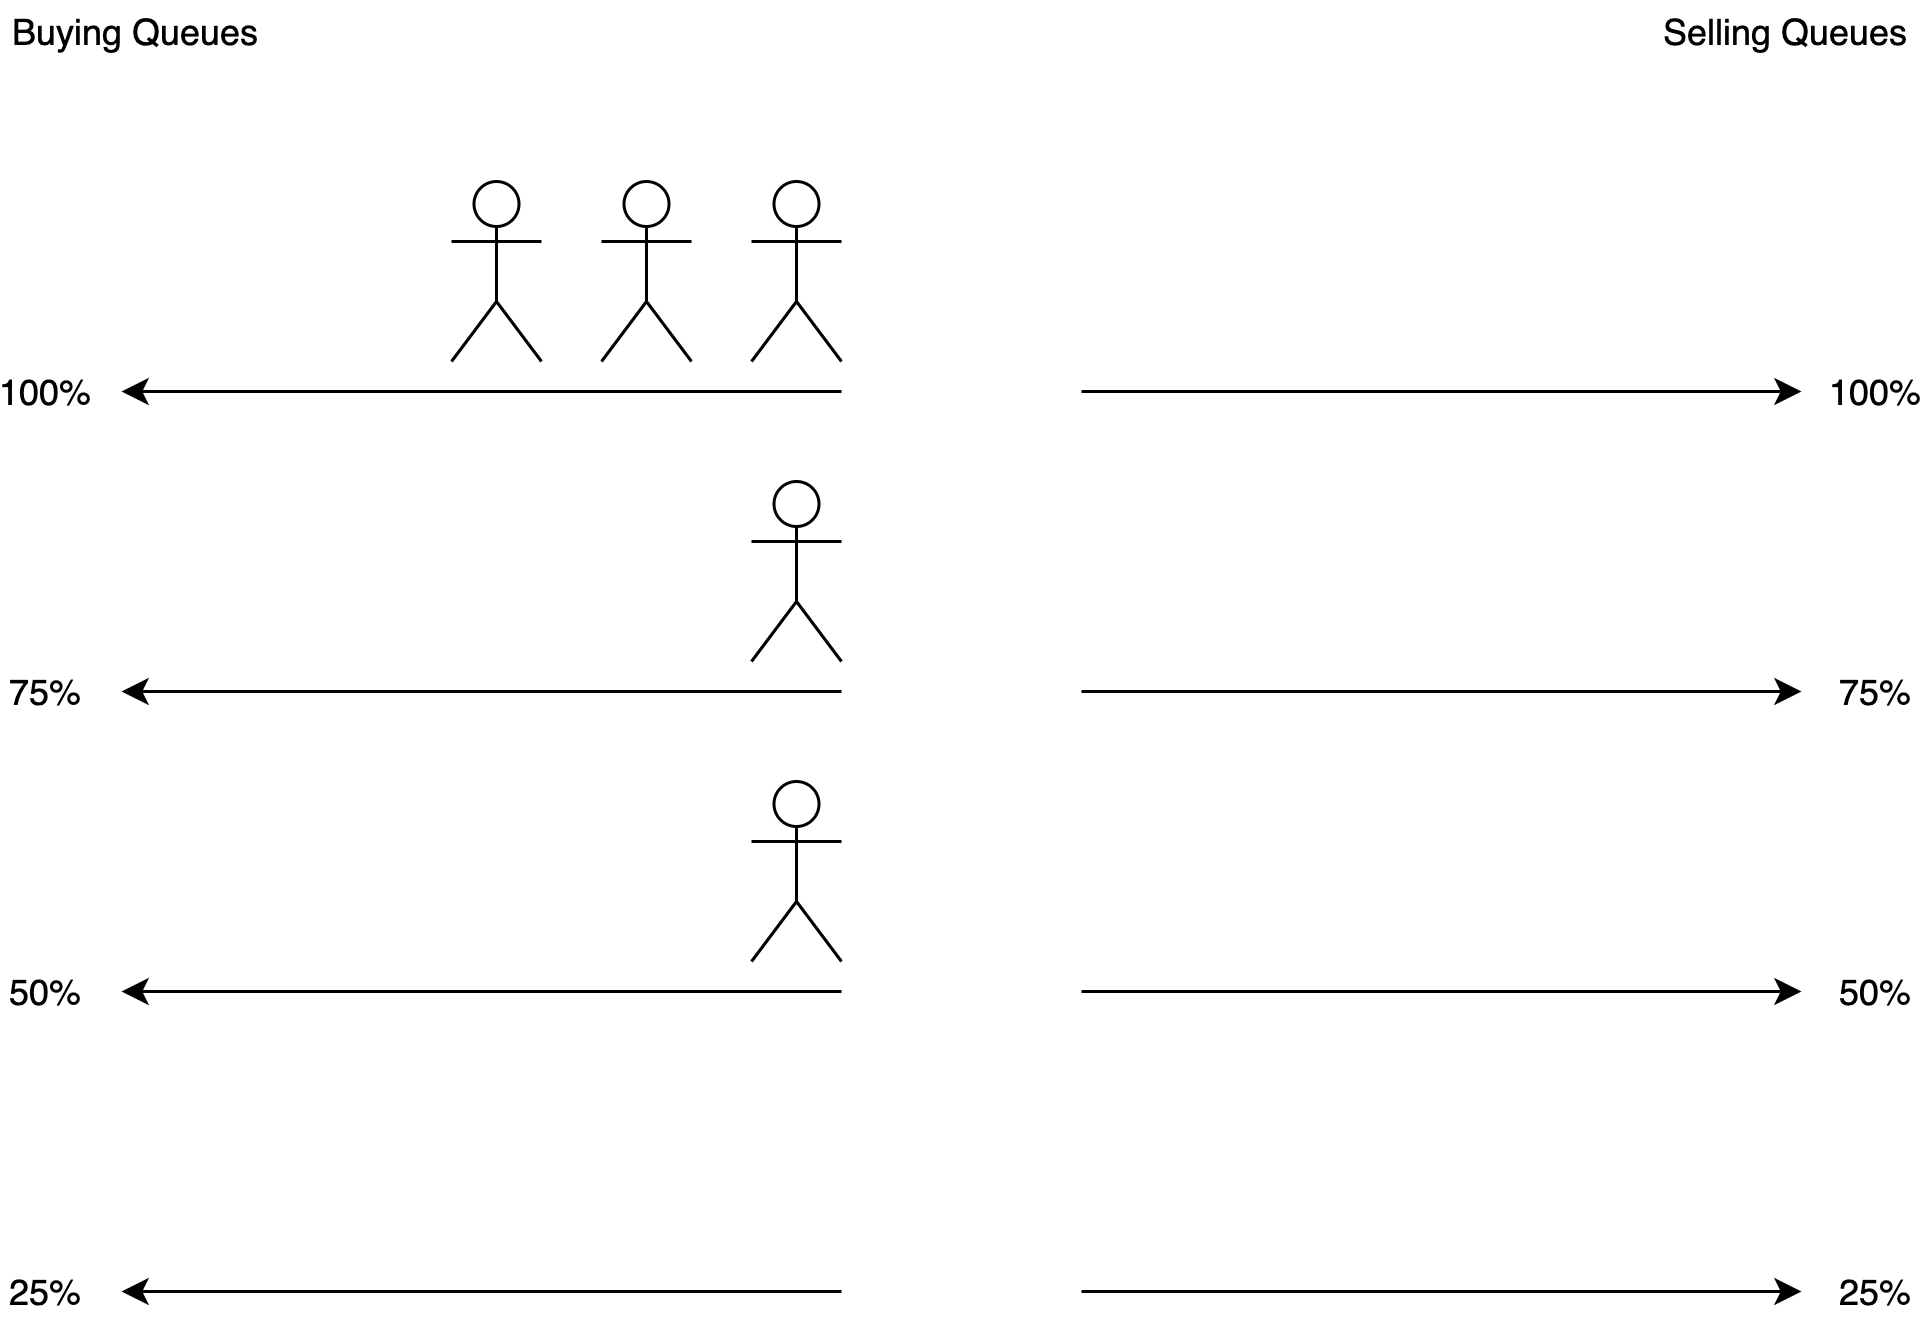
\includegraphics[width=12cm]{figures/aftermarket-high-demand.png}
    \caption{Aftermarket with high demand}
    \label{fig:aftermarket-high-demand}
\end{figure}

Contrarily, the same state can occur in the selling queues. Meaning that the supply is higher than the demand. A buyer can instantly fill a sell order.

It is also possible that the aftermarket levels at a lower price than the original ticket price. This is shown in Figure \ref{fig:aftermarket-mixed} where multiple people are willing to sell the ticket for 75\% of the original price. On the other side, multiple people are willing to buy a ticket for only 50\% of the original ticket price. In this state, any seller could immediately settle a trade at 50\% of the original price and any buyer could immediately fill an offer at 75\%. 

\begin{figure}[H]
    \centering
    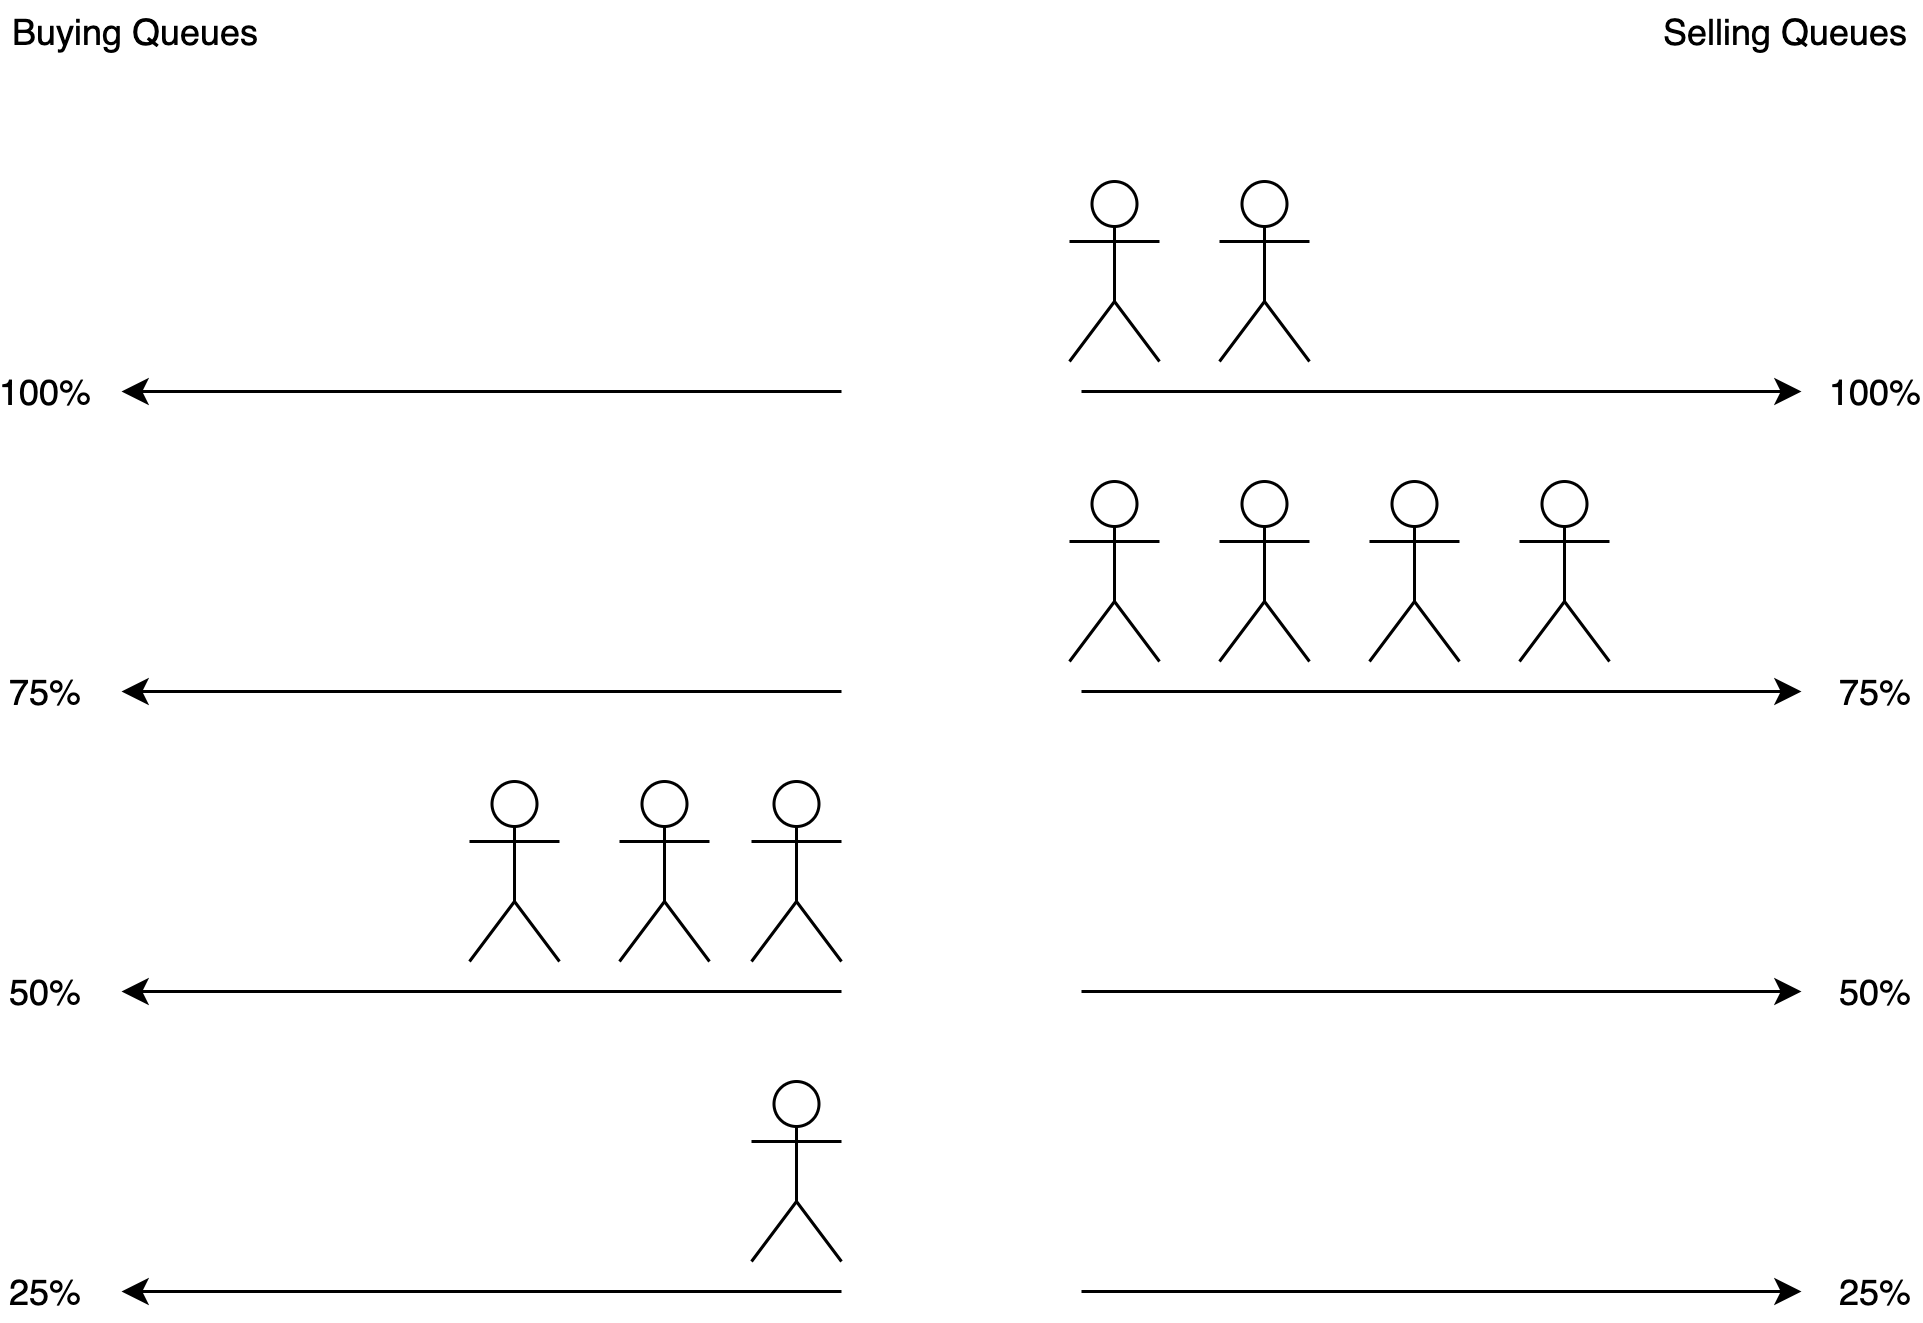
\includegraphics[width=12cm]{figures/aftermarket-mixed.png}
    \caption{Aftermarket with lower prices than original ticket price}
    \label{fig:aftermarket-mixed}
\end{figure}

Another scenario that is possible can occur when people join the wrong queue. This can occur when a sell and a buy order is processed in the same block or due to wrong interaction with the SC. Such a state of the aftermarket is shown in Figure \ref{fig:aftermarket-arbitrage}. There is a person willing to sell a ticket for less than the highest offer on the buyer side. This opens the possibility of arbitrage trading. A third person can buy the ticket at 50\% and immediately resell the ticket again for 75\%. 

\begin{figure}[H]
    \centering
    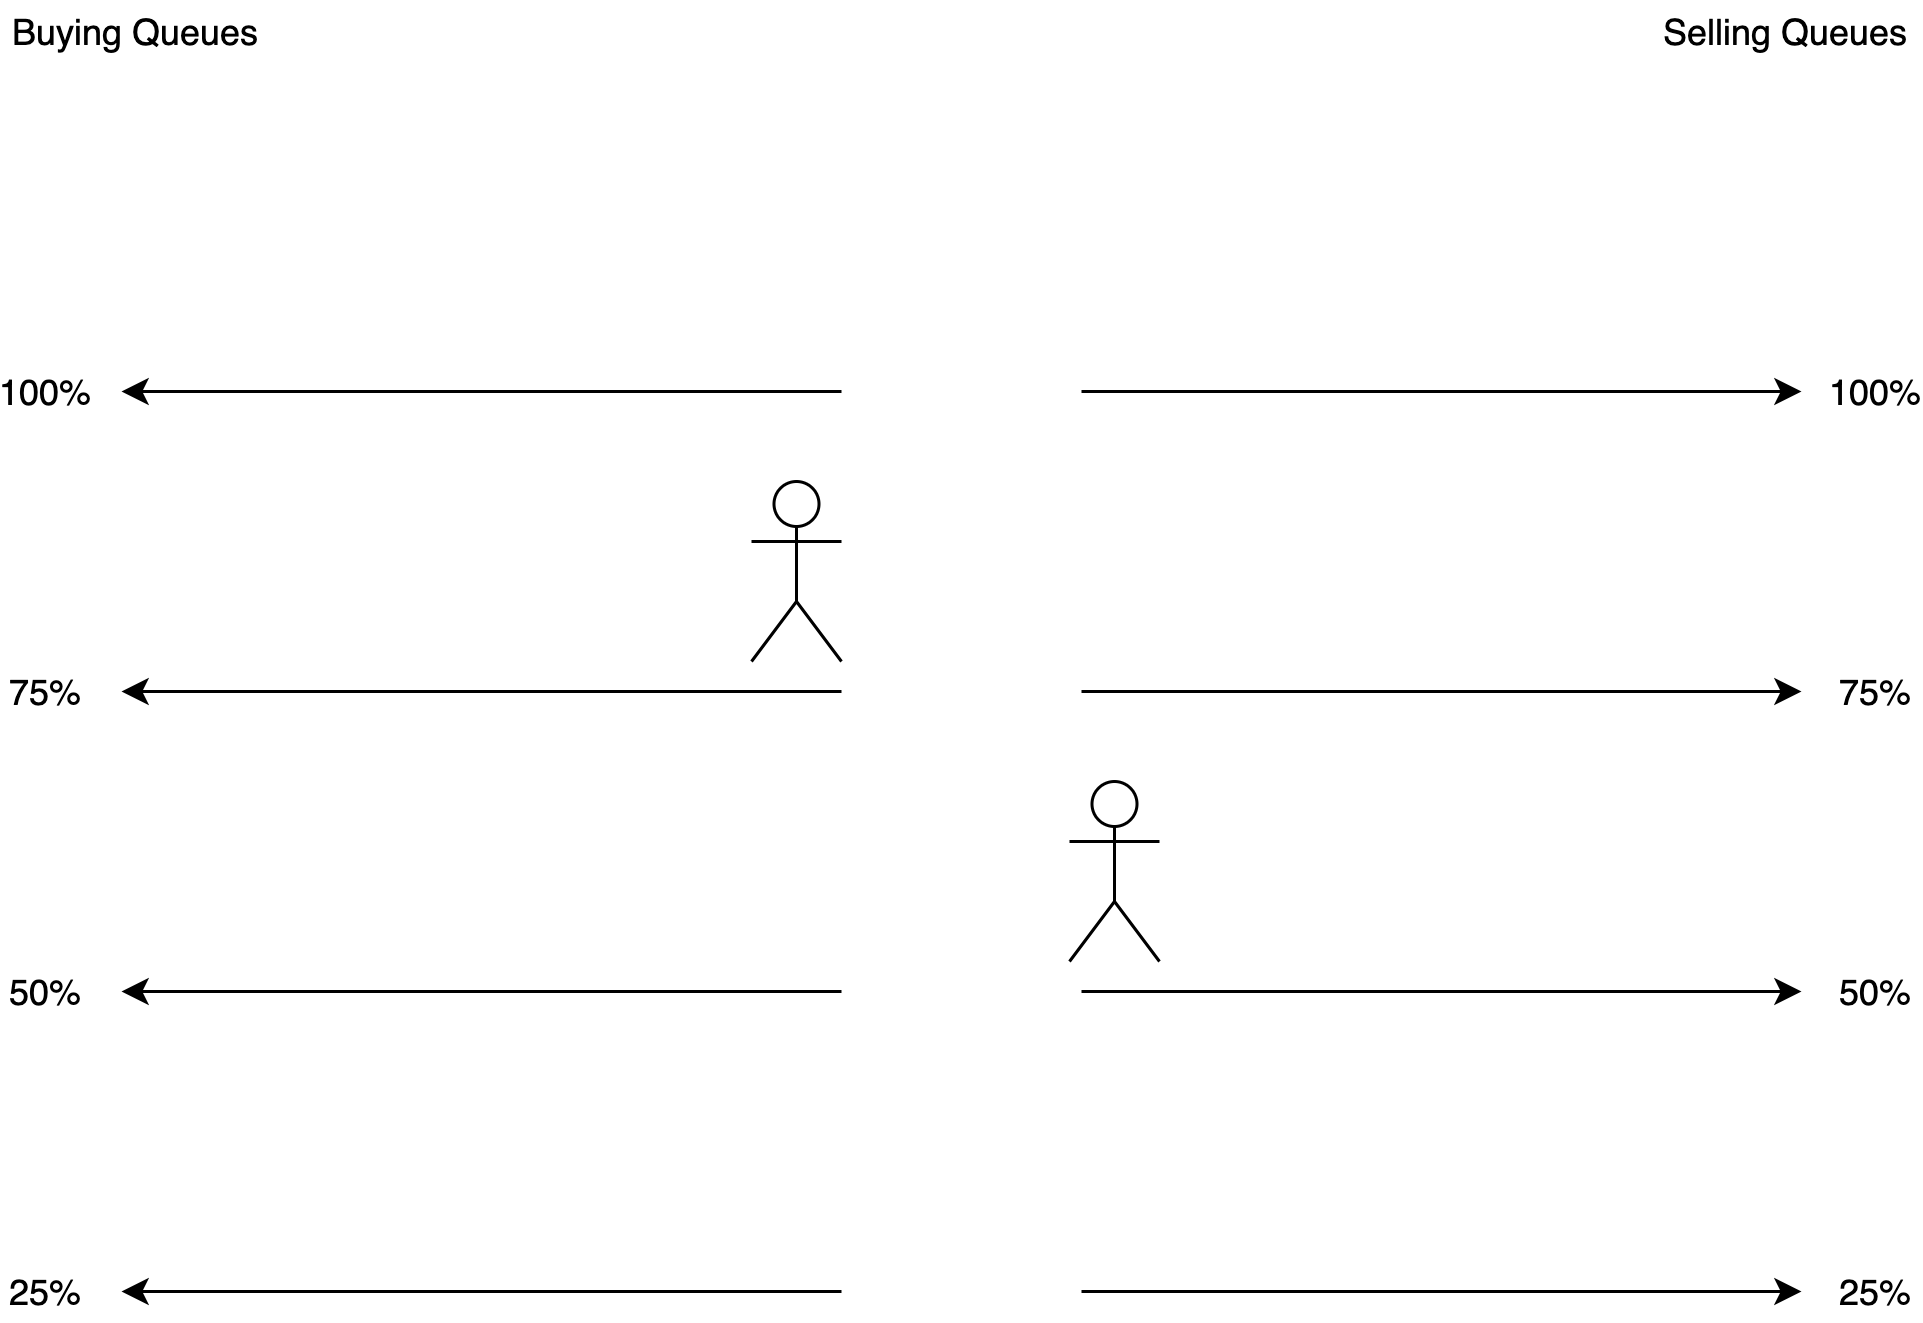
\includegraphics[width=12cm]{figures/aftermarket-arbitrage.png}
    \caption{Aftermarket with arbitrage opportunities}
    \label{fig:aftermarket-arbitrage}
\end{figure}

There are two solutions to solve that problem. Joining the wrong queue due to human error can be eliminated by warning the user in the frontend application that joining the selected queue results in a loss of opportunity cost. 

Solving the issue in the SC comes at the price of efficiency. Additional parameter can be introduced to keep track how many people are in each queue. Before each trade, the SC evaluates if the described state occurs. However, depending on the granularity of the queues, it might not be feasible to loop over each queue as this results in higher network fees and might lead to an 
\textit{out-of-gas exception}.

In this project, a warning in the frontend is displayed when a user attempts to join a queue that is not optimal.

\subsection{Presale}\label{section:des:presale}
Whenever an event takes place and the demand for the tickets is high, the potential guests will try to buy the tickets when the sale period starts. This leads to a high traffic on the ticket sellers website. It is then also not clear, which person can finish the buying process and is often determined by the internet speed of their internet service provider.

To prevent this problem and to have fair and clear odds for every guest, a lottery system for the initial ticket distribution is put in place. Every guest, that wants to attend the event, can place a buy order during the presale. This order will cost as much as the ticket. At the end of the presale period, the tickets will be distributed using a random number, in the case a guest has not won a ticket, he then will be able to reclaim the spent money. If there are more tickets than interested buyers in the presale, each of them receives a ticket. 

The design pattern of the \textit{future blockhash} is used to generate a random number. During the creation of a presale ticket type, a future blocknumber is defined. This block acts as the closing date for the presale as well as the source of randomness. This design patter is a good fit due to its simplicity. There is a chance of manipulation by the miner that adds the block with the defined number by not publishing a block if randomness is not in his favour. However, in order to do so, the miner must resign on the block reward. If this is an actual threat to a ticketing platform, the prices have to be larger than the ticket price. 

\subsection{ERC Standard}
All three ERC standard explained in Section \ref{subsubsection:token-interfaces} require a function which allows the owner to transfer the token/ticket to another address of his choice. Without explicitly deactivating this function, people are able to sell the ticket on a different platform for higher prices and consequently, allowing a secondary market to emerge. The goal of this project is that there exists only one marketplace/exchange for each event operating transparently on the BC. Also, tickets must not transferred in the same way as these ERC standards do.

It is be possible to deactivate the transfer function or whitelist a specific exchange address such that tickets could only be sold through this exchange. However, this breaks the design principle of these ERC standards. These standards are developed to create a common interface such that a token can be used across multiple exchanges and the usability is the same among different tokens. Also, tickets must only be resold in one contract to minimize the risk of emerging a black market (as described in Section \ref{section:aftermarket}). Merging the event logic with the aftermarket logic in one contract has a positive side-effect that no extra transaction is needed to approve the aftermarket (DEX). 

Furthermore, the logic for approving and storing other exchanges increases the complexity of the event SC and becomes more expensive to create and deploy a new event.These are the reasons for not implementing any of the ERC interfaces for the event contract and instead creating a new contract from scratch. 


\subsection{Economics}\label{design:economy}

The economic model works differently in a decentralized system. The entire business logic is stored in public SC that anybody can fork and redeploy. With the proposed design an event host does not need any hardware or software infrastructure to create an event and issue tickets. However, other stakeholders play a crucial role in the ticketing process as shown in the diagram \ref{fig:dlt-based-landscape}.

The host either relies on trustworthy identity approvers or does his own KYC procedure. To incentivize identity approvers to become trustworthy and to compensate them for their service, a fraction of each ticket price is directly paid to the selected identity approver. Since this is an open design identity approvers compete with others to become popular among the event hosts.

Furthermore, the same principle applies for the graphical user interface (GUI) builders. Anybody can interact with the SC. This can either be done directly with the command line interface (CLI) or using a GUI. A GUI provider is also compensated for his service if the ticket is bought through his application. This creates a fair competition among different GUI builder.

Affiliates are companies or influential people that promote an event. Affiliates are also included in the buying process and are being compensated with a direct payment for each ticket that is bought due to their service. 


\begin{figure}[H]
    \centering
    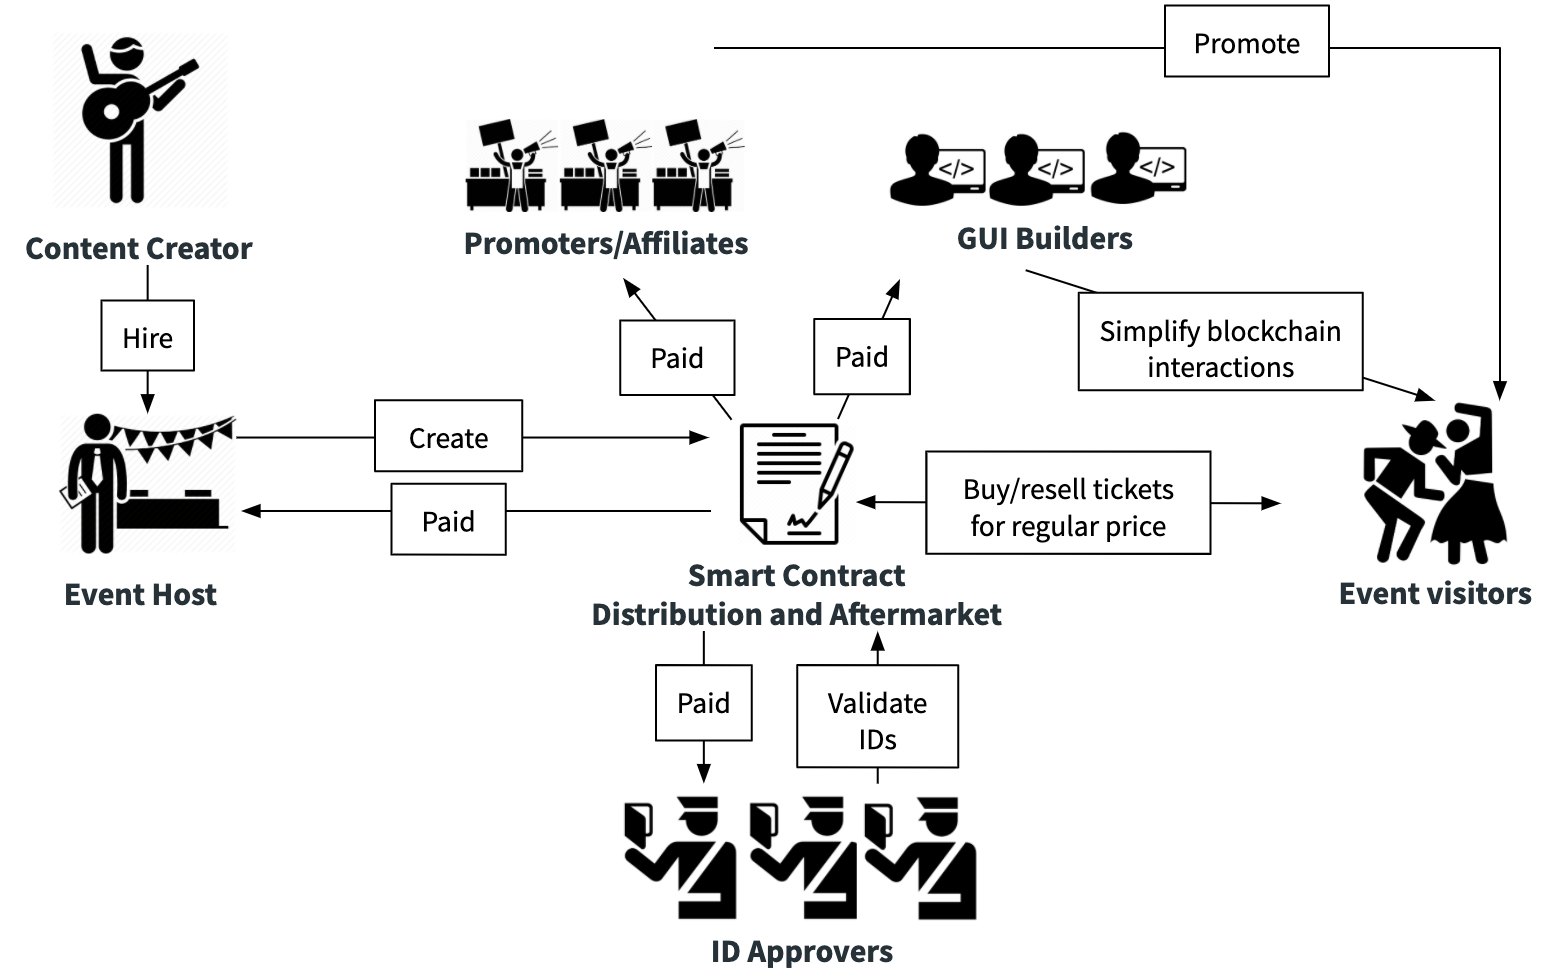
\includegraphics[width=16cm]{figures/dlt-based-landscape.png}
    \caption{DLT-based architecture}
    \label{fig:dlt-based-landscape}
\end{figure}


% author: Simon Bachmann

\section{Social Trust Certificates}\label{section:social-trust-certificates}

A decentralized ticketing platform does not restrict any user from creating an event on the DL. Thus, a mechanism must be developed to mitigate fraudulent events.

A common design pattern for this problem is an on-chain voting mechanism as explained in Section \ref{section:blocktix}. Usually, these decentralized platforms create a multi-purpose token for this. One of the tokens functions is governance. Token holders are eligible to cast votes if they think an event is fraudulent and in return they receive maintenance fees. However, this requires that the event creator must deposit some currency when creating an event. Furthermore, people must make an on-chain transaction to vote on suspicious events. This makes the UX more complex for the event host. Introducing a new token for every decentralized app also results in a fragmented ecosystem.

The goal is to enable users to check whether an event is legitimate or not without the need of a governance mechanism. Furthermore, the level of trust that is needed from third parties must not be greater than in the current ticketing ecosystem. 

\textit{Social trust certificates} enable a user to check whether the event is legitimate or not without the need of a third party. Event hosts upload the same public key, that is used for creating the event, to a social profile or the official event website. This way, an event host can proof his ownership of the event as well as the social profile or website. 

Event guests can retrieve the URL of the website or social profile from the SC and then verify themselves, if the event is legitimate or not. However, this is not 100\% foolproof. For an imposter it is easy to fake an official website with a slightly different URL and buy followers on social media platforms. However, this threat already exists today. Aggregating multiple social media platforms makes it harder for an attacker and thus, increases the legitimacy of an event compared to today's standards. 

Figure \ref{fig:trust-certificate-event-website} illustrates how the event host can use the official event website to increase the authenticity of the event. 

\begin{figure}[H]
    \centering
    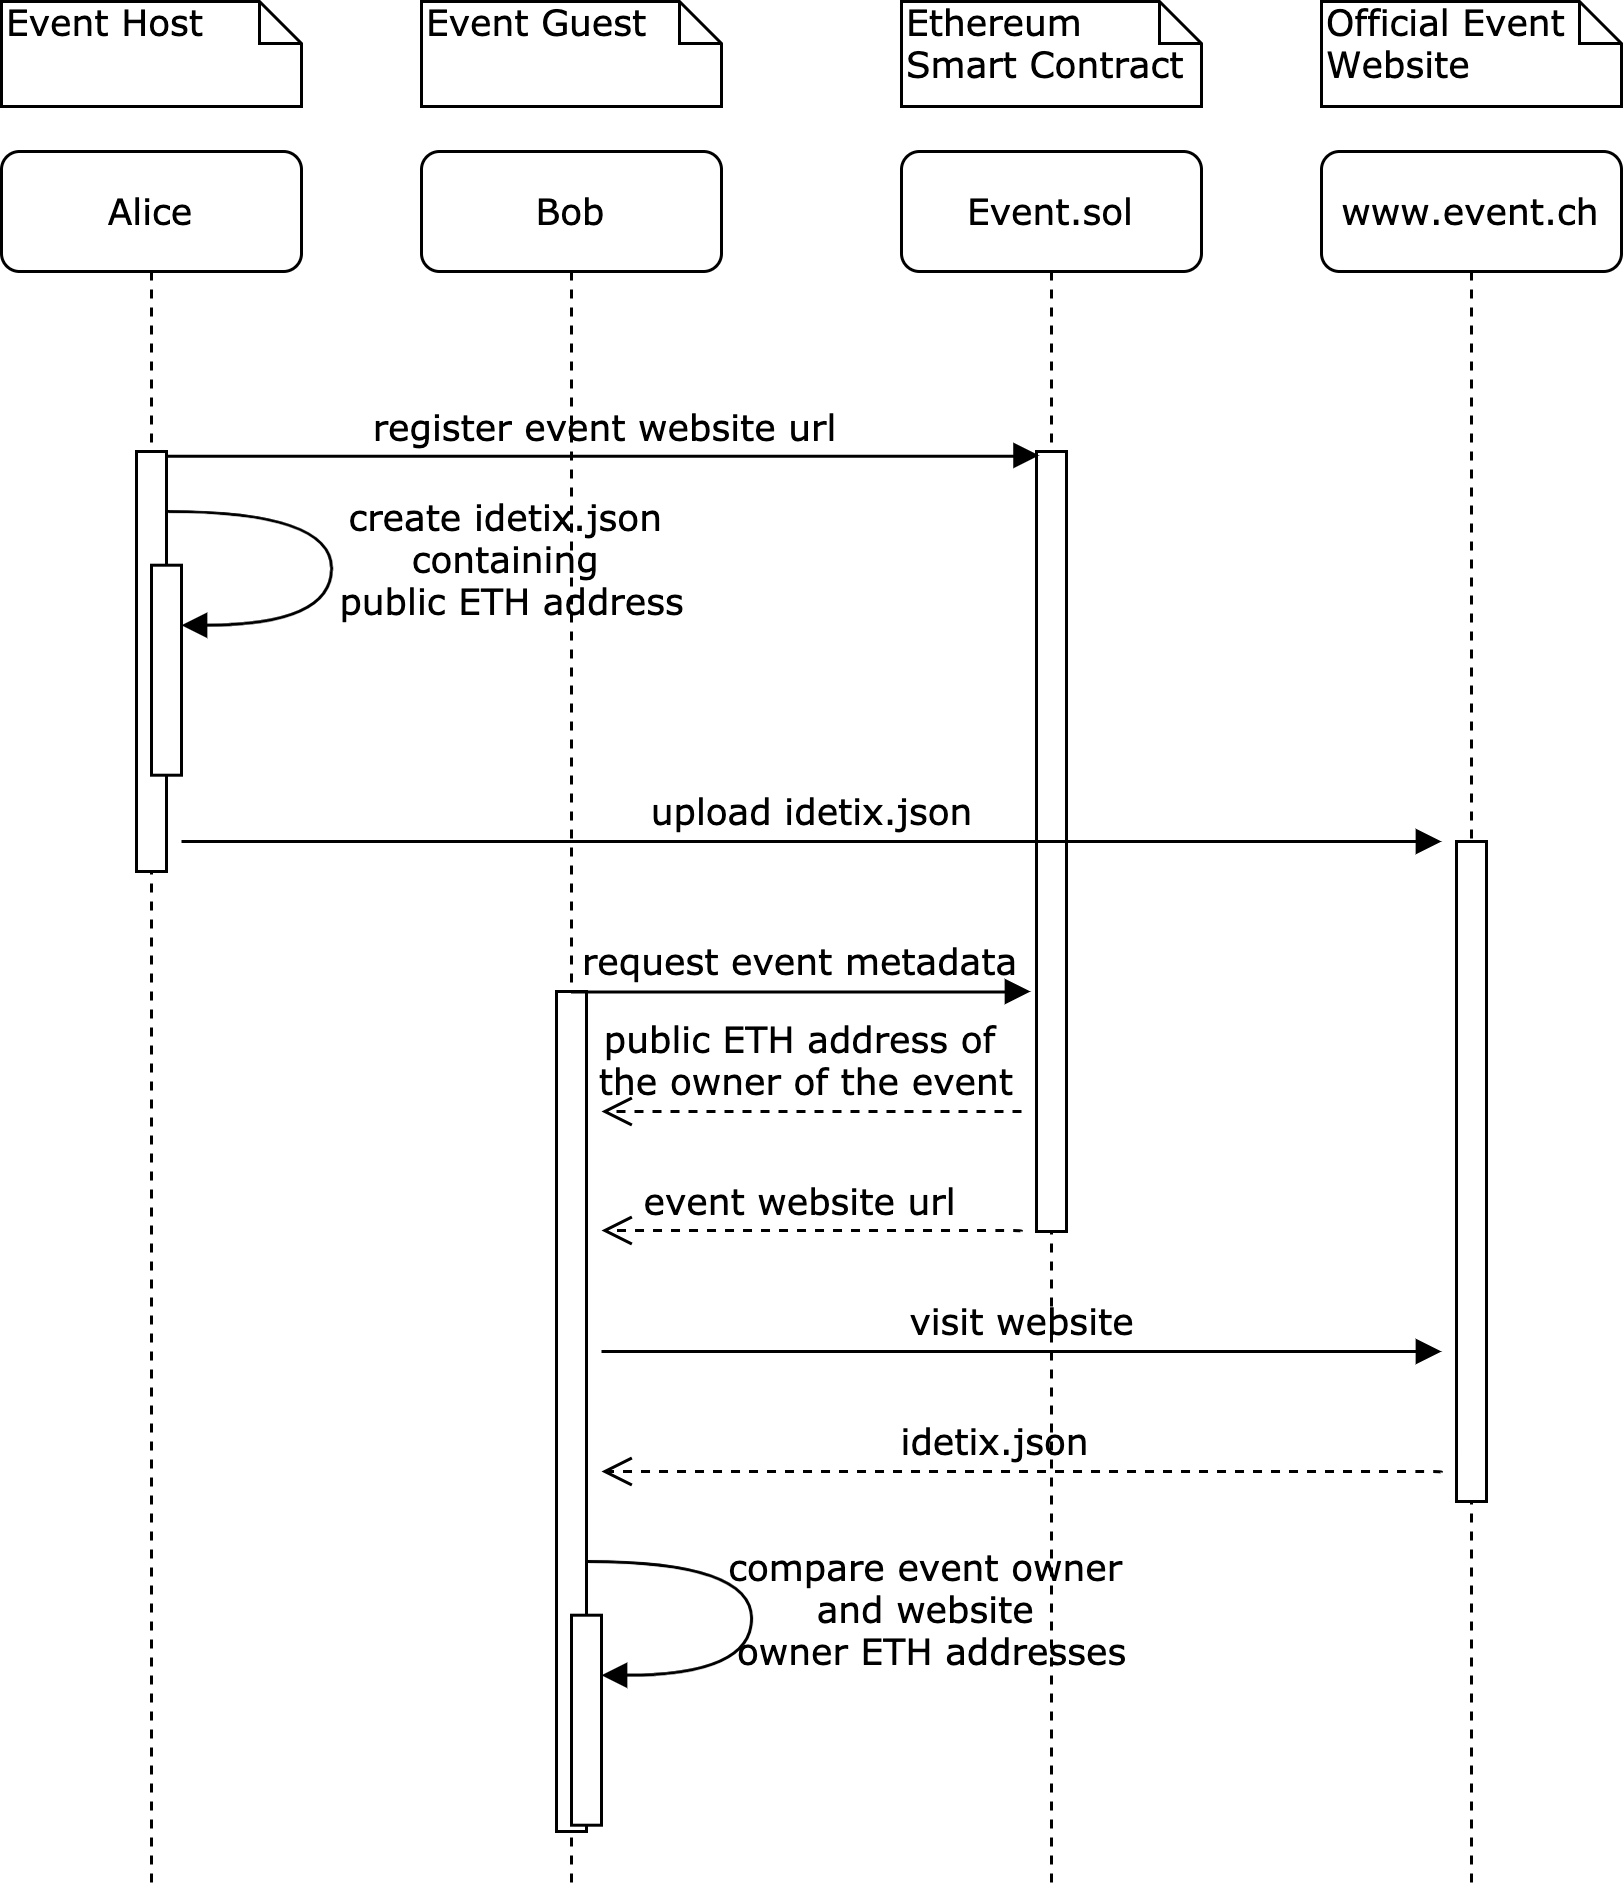
\includegraphics[width=14cm]{figures/social-trust-certificates.png}
    \caption{Social trust certificated on the event website}
    \label{fig:trust-certificate-event-website}
\end{figure}

Similarly, this procedure can be applied to any social profile such as Twitter, Facebook, Instagram and other social media platforms. Instead of uploading a JSON file or HTML meta-tag to the website, the public address is included in the profile description on that particular social media platform. 
\section{Identity Approver}
% author: Nicolas Spielmann

The core idea of the Identity Approver is to allow guests to verify claims of ownership over an identity and store the linked Ethereum address with the provided identity, once the verification process was completed successfully. This is, to avoid the misuse of identities such as using it multiple times. In the following section, the concept of Identity is described.

\subsection{Identity}\label{design:identity}
Since the goal of the project was to come up with a decentralized ticketing platform, a decentralized design of identity was needed. Therefore, following approach of identity and identity verification was provided.

Identity is a chain of claims and proofs. For example, to obtain a passport for a newborn child, the birth certificate of the child is required. In this example, the birth certificate is the proof. The government then uses this proof, checks it and then issues the requested passport. As it is not feasible to request the birth certificate of every event guest, it is suggested to use something, that goes through a KYC-Process when obtaining it. One of these products would be a phone number, since those can only be obtained when providing an identity. Therefore we can verify an identity of a guest by checking, whether he has ownership over the phone number he claim is liked to his identity. Once this check is successful, the level of identity verification of the linked Ethereum address is set on the identity SC. This has the benefit of only needing to store integers that represent a level of proof linked to the Ethereum address. Confidential data is only stored off chain at the identity approver.

To achieve a decentralized solution for approving identities, it was suggested to automate this identity approving process and allow everybody to act as an identity approver. Therefore, everybody can register itselfe on the identity SC as an approver and also use its own idea and implementation of identity proofs.
This leads to the host having to decide, which identity approver he wants to use for his event. 

\subsection{Sample Design}
For the scope of the project, the idea was to provide an easy to run example implementation of this automated identity approver application. The sample implementation knows three different levels of identity.

\begin{itemize}
    \item The first level is verification by an email address. To verify the ownership, the application uses the in Spring included mail implementation. The mail address and its credentials are set in the application properties. For testing purpose, a dedicated gmail address has been created and used to send the random sequence via mail.
    
    \item The second level of identity is verification of a phone number. To send text messages to a phone number, Twilio is used. Twilio provides an easy to use API for Spring Boot, that can be used to send text messages. 
    
    \item The third level of identity verification is a KYC-like process. It requires the user upload a picture of the machine readable part of his passport, a picture of the whole passport and a selfie. The OCR(Optical character recognition)-Software Tesseract\footnote{\url{https://en.wikipedia.org/wiki/Tesseract_(software)}} is used to extract the text from the machine readable part of the document and the correctness is checked . Afterwards the similarity of the picture on the passport and the selfie is calculated using AWS. 
\end{itemize}





% author: Claudio Brasser

\section{Guest Client}\label{section:guest client}
The Guest Client is the web-based application that allows a user of the ticketing platform to interact with the smart contracts and the ticketing platform as a whole. It focuses on delivering a consistent \& user-friendly interface for mobile devices. The following section will briefly introduce the main building blocks of the application.

\subsection{Views}

The application consists of four main views. While the application is started for the first time, the user is granted to connect to a cryptocurrency wallet application. Initially, this procedure was handled seamlessly by the \textit{walletconnect} library. Due to a breaking bug in this library, this is not possible at the time of writing. There is a fallback method to connect wallets via \textit{metamask}.

The user is first greeted with a geographical map \ref{img:event-map}, containing pins at each of the locations at which an event is currently registered. These locations are provided by the event host via a city or address name and are then translated into geographical coordinates using a \textit{reverse geocoding service}. If the event host chooses to not provide a location, his event will not show up on the map. 
\begin{figure}[H]
    \centering
    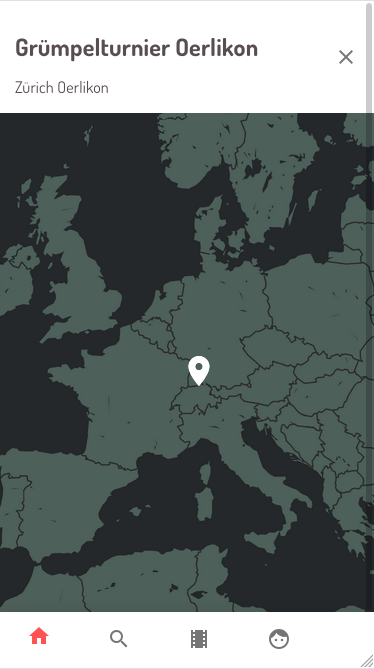
\includegraphics[width=7cm]{images/map.png}
    \caption{Event Map \protect\footnotemark}
    \label{img:event-map}
\end{figure}
In the second tab of the application, all events are displayed in a conventional list format \ref{img:event-list}. Here they can be filtered through a search bar, which performs a full text search on all the event properties. This enables searches by various properties such as location, title, and type all through the same search field.

\begin{figure}[H]
    \centering
    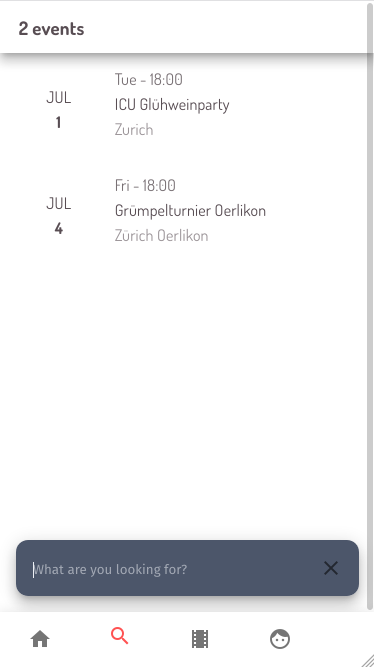
\includegraphics[width=7cm]{images/event_list.png}
    \caption{Event list}
    \label{img:event-list}
\end{figure}

When a user selects an event through one of the aforementioned views, he is taken to the event detail \ref{img:event-details} page. This is the most information-rich view of the application, since it contains most of the smart contract interaction possibilities. First presented is all of the information on the event, as well as the identity approver chosen by the event host, if any. Further down, the user can see a graphical representation of all ticket categories. The user can buy any of the available tickets by tapping on the desired category/seat and submitting the appearing pop-up. If the event is still in its \textit{presale phase}, the user can also join the presale from within this view. 
\begin{figure}[!tbp]
  \centering
  \subfloat[Event Information]{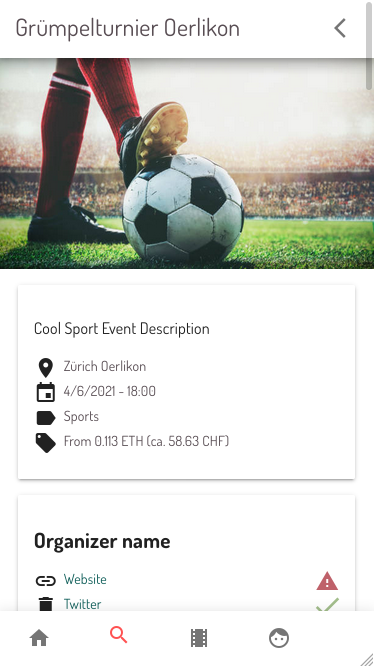
\includegraphics[width=0.3\textwidth]{images/event_1.png}\label{fig:f1}}
  \hfill
  \subfloat[Seating Plan]{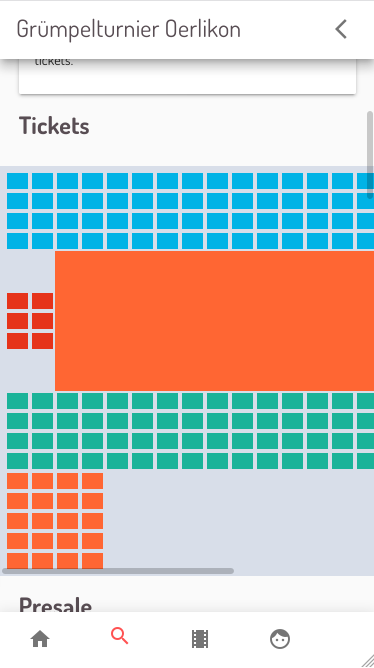
\includegraphics[width=0.3\textwidth]{images/event_2.png}\label{fig:f2}}
    \hfill
    \subfloat[Aftermarket]{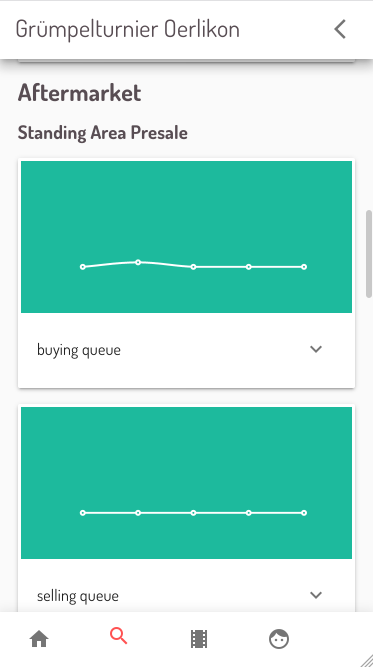
\includegraphics[width=0.3\textwidth]{images/event_3.png}\label{fig:f3}}

  \caption{Event Detail View}
  \label{img:event-details}
\end{figure}
Lastly, the aftermarket state is shown for each ticket category. This is done via line graphs, showing each queue as described in \ref{section:aftermarket}. For the \textit{buying queues}, the user can directly enqueue or buy an aftermarket ticket if there are offerings in the selling queue. The selling queues can be joined from the inventory view, as described later on in this section.

The third section of the application displays the tickets bought by the user and joined presales. For each ticket, the user can open a modal content window, showing all relevant ticket information by clicking on the ticket. In addition to all information regarding the event and the specific ticket, the user can also choose to sell his ticket from this view.
\begin{figure}[!tbp]
  \centering
  \subfloat[Ticket List]{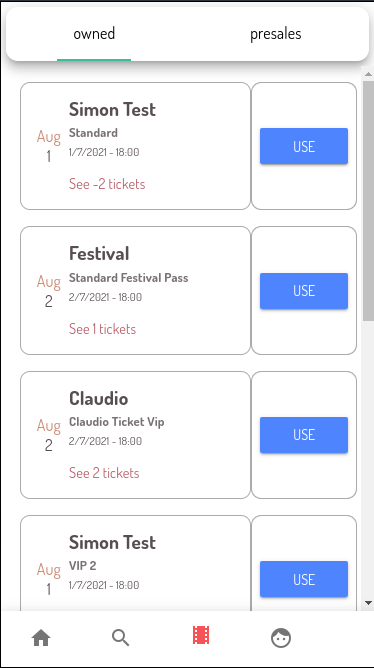
\includegraphics[width=0.4\textwidth]{images/in_1.png}\label{fig:f1}}
  \hfill
  \subfloat[Ticket Details]{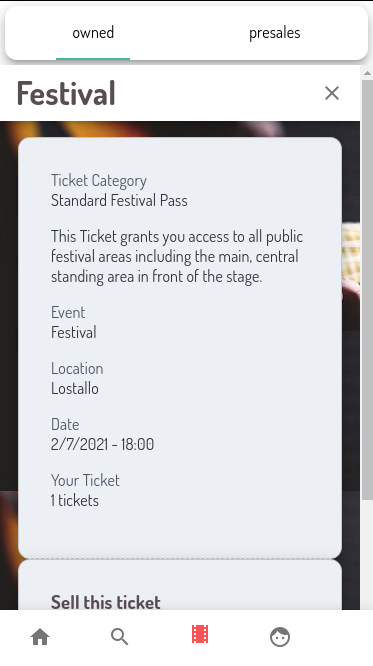
\includegraphics[width=0.4\textwidth]{images/in_2.png}\label{fig:f2}}
  \caption{Inventory view}
  \label{img:inventory}
\end{figure}

In the last tab, information regarding the identity approval status with all registered identity approvers is shown to the user . For each approver, the levels of authentication are displayed in increasing order of severity, as well as the users current level of authentication. Since each event can use any registered third party as approval service, there might exist identity approvers with their own, external approval services. For these, the user has to inform himself via the information provided by the respective event host on how to reach the necessary level of authentication. \\
If an event host has chosen the \textit{Idetix Identity Approver} for his event, the user can complete the approval process from within the application. This is done via one of the methods described in [Ref]. 
\begin{figure}[H]
    \centering
    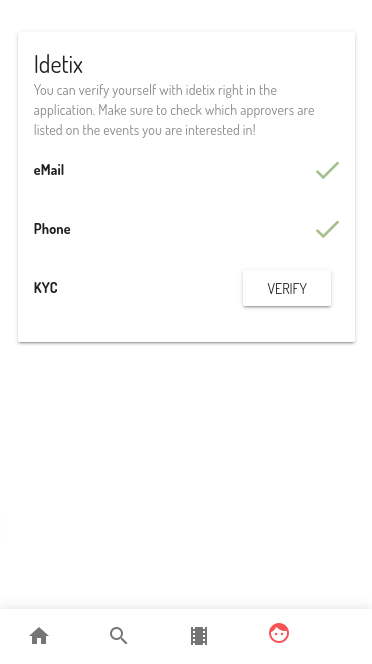
\includegraphics[width=7cm]{images/ide_1.png}
    \caption{Identity approval view}
    \label{img:identity}
\end{figure}


%Author: Michael Bucher
\section{Host Client}

The host-client is a web-based application for event hosts to edit, track and create events. The application contains one component that is displayed and runs all the time. This component shows the active view and it contains a permanent navigation bar (Figure \ref{img:host-client-navbar}) that routes between the views of the application. The application is structured into five views. One of them, the event summary view, can be reached by clicking on an existing event card on the landing page and the other four can be reached through a sidebar. The navigation bar contains a button on the top left that toggles the sidebar (Figure \ref{img:host-client-sidebar}). It allows to route to the event list (landing page), a form to create a new event and as third option either a form to register as ID approver or, if already registered as ID approver, a form to approve an account manually.

\begin{figure}[H]
    \centering
    \fbox{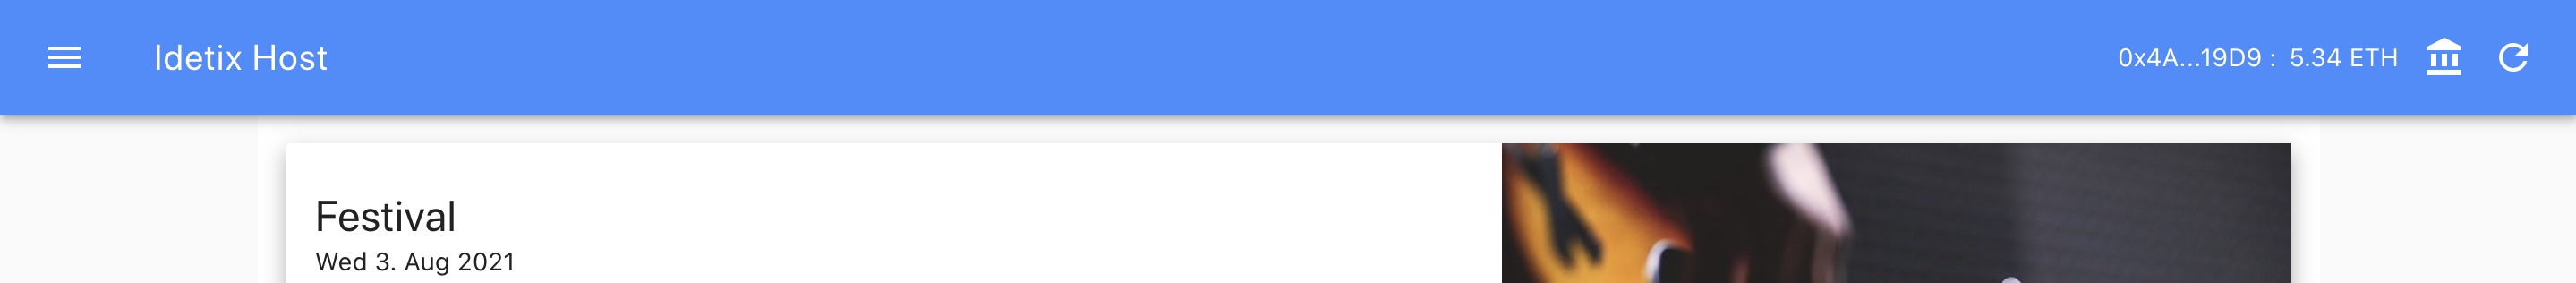
\includegraphics[width=15cm]{images/host-client-navbar-screenshot.png}}
    \caption{Host-client navigation bar \protect}
    \label{img:host-client-navbar}
\end{figure}

\begin{figure}[H]
    \centering
    \fbox{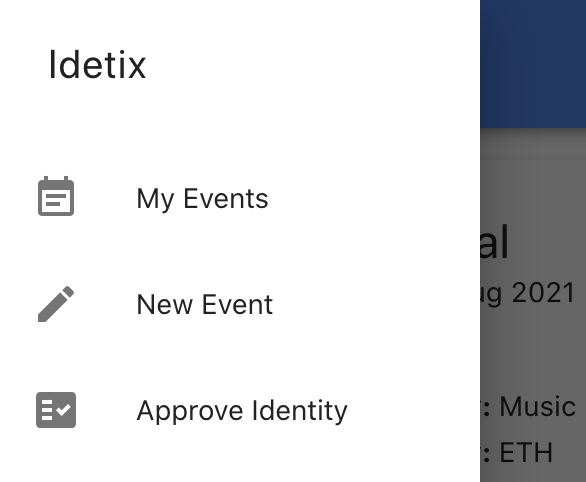
\includegraphics[width=5cm]{images/host-client-sidebar-screenshot.png}}
    \caption{Host-client sidebar \protect}
    \label{img:host-client-sidebar}
\end{figure}

When the application is started for the first time, the application needs to connect to a cryptocurrency wallet like Metamask\footnote{\href{https://metamask.io/}{https://metamask.io/}} to establish a connection to the Ethereum BC. The user is prompted to connect the wallet with their accounts to the website. As soon as the wallet is connected, the base component loads all registered ID approvers and all events that are owned by the active account in the wallet. Upon loading the main event data, the event list view is displayed, showing a list of the existing owned events. To create a new event, the event creation form is accessible through the navigation sidebar.

\subsection{Event Creation}\label{design:event-creation}
The event creation form component contains various input fields to set up a new event. There are parts that are required, like the title, location, date, description and the aftermarket granularity. Only when those required parts are filled, a button is shown at the bottom to create the event. An ID approver is not required based on the design of the event factory contract. Further, an image, a website or twitter account are also optional.

When selecting an ID approver, their selector is automatically filled with the existing ID approvers that are registered on the identity SC. When an ID approver is selected, the level selector on its right is updated with the according methods. Further, to get more information for the selected ID approver, the question mark icon on the right opens a dialog window that explains the involvement of an ID approver to this event and also leads to a dialog that provides an overview of the ID approver, like its website, twitter and what identity verification methods are supported.

Further, the website and twitter input fields show the status of the trust certificate (see Section \ref{section:social-trust-certificates}) check for the given input and the active account. This way, a correct integration of a host's certificates can be checked. Finally, upon creating an event, the user is routed back to the event list.

\begin{figure}[H]
    \centering
    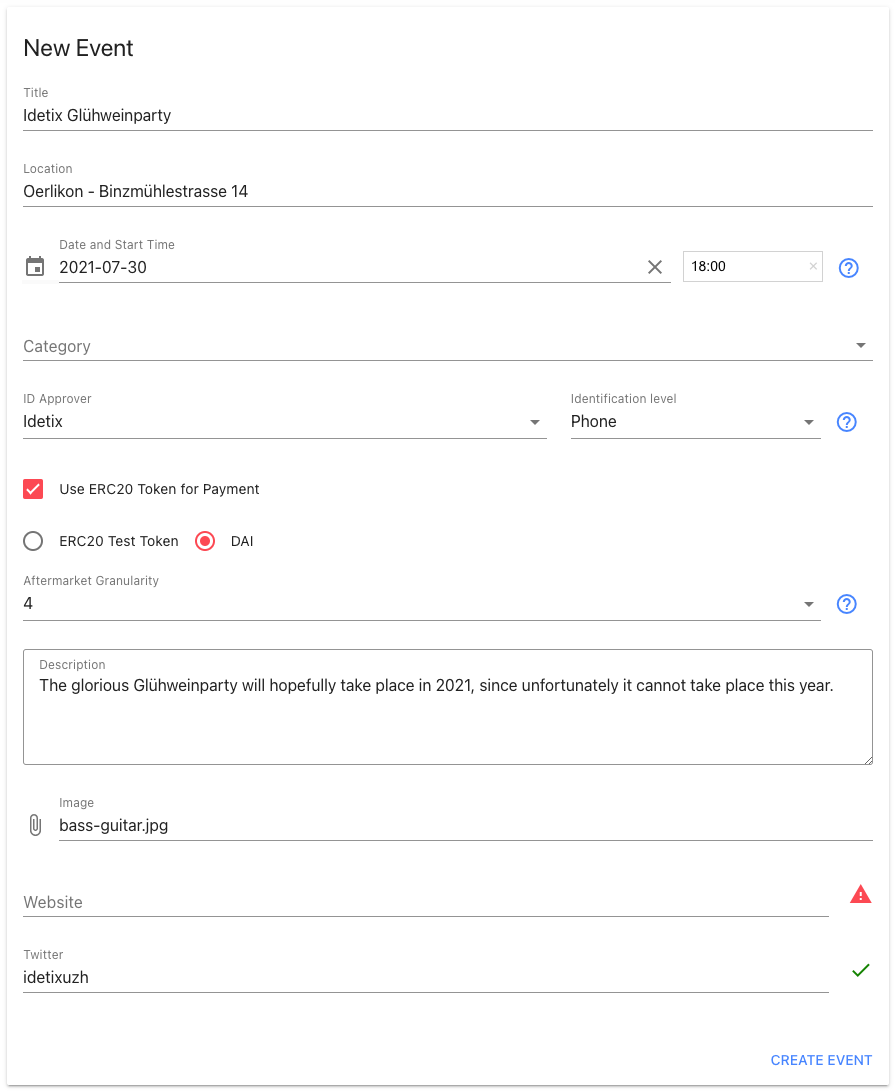
\includegraphics[width=15cm]{images/host-event-form.png}
    \caption{Event creation form \protect}
    \label{img:host-event-form}
\end{figure}

\subsection{Event List}
The event list is a simple view that contains a list of event cards. These event cards contain the metadata for the according event and some information directly fetched from the BC, i.e. the maximal number of tickets per person, the currency, or the ID approver that is required to buy a ticket. For more information about an event, a click on the card routes to the event summary view.

\subsection{Event Summary}
The event summary view (Figure \ref{img:host-event-summary}) contains multiple components that offer an overview of the event, its tickets, and their states. A slightly reconfigured event card to the card in the event list is shown on top. Here it also shows the event contract address and an edit button. Either the metadata or the maximal number of tickets per person can be changed. Upon clicking the edit button, the host is prompted what to change and the according component is shown to make such a change.
When editing the metadata, an event creation form is displayed that is filled with the current metadata. This form can be edited and then submitted. In the form, only the image input is not filled out with the current data, since it is stored in a Base64 representation. If no new image is uploaded in this input field, the current image is just used again. After a change to the event, the event summary is shown again with the updated data.

\begin{figure}[H]
    \centering
    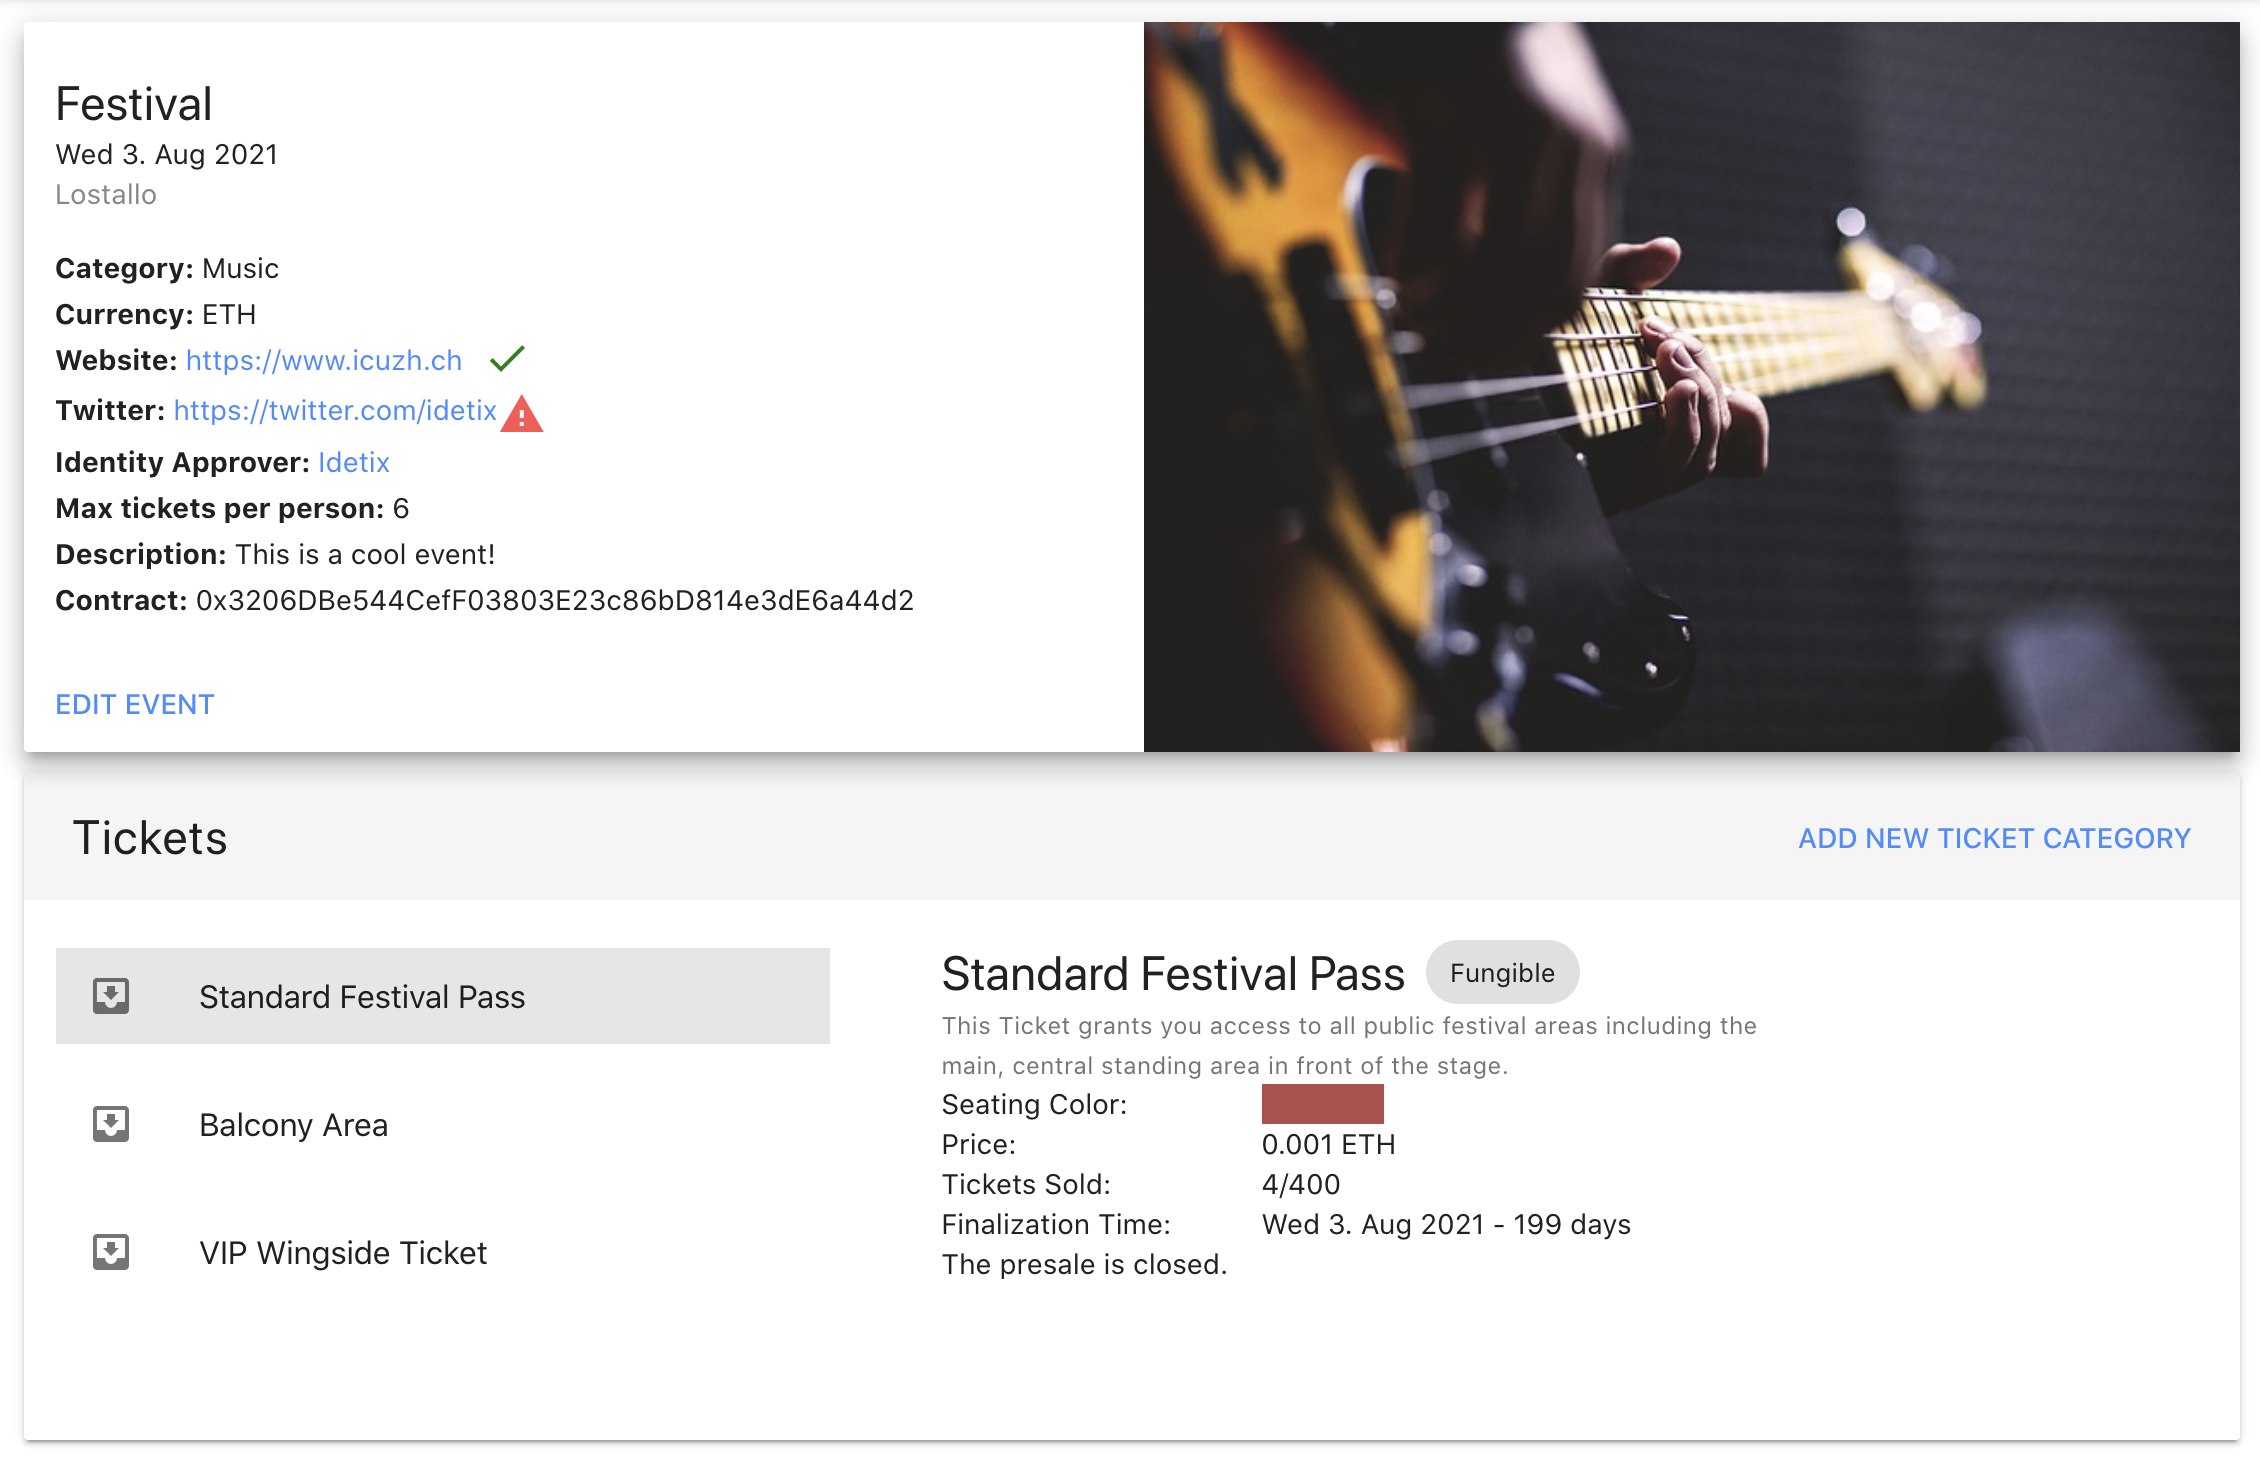
\includegraphics[width=14cm]{images/host-event-summary.png}
    \caption{Event summary view \protect}
    \label{img:host-event-summary}
\end{figure}

Below the event card, the tickets of the event are summarized. On the left is a list of ticket types that exist for that event and when selecting a ticket, the information about this ticket is shown on the right. This information contains data from the BC and the metadata that is fetched from IPFS. It shows details such as whether the ticket is fungible or non-fungible, the price, the amount of tickets that have already been sold and the finalization time. This finalization time specifies the time, when tickets can no longer be bought or sold.
Tickets with a presale further show the status of this presale. Either, the presale has already passed, or otherwise, an estimated time is shown, when the presale presumably will end.

Additional to that, the BC information of a ticket and the ticket's metadata which is stored on IPFS is shown, i.e. title, description and the seating color. The latter may then directly be used to visualise what seats this type contains on the seating plan that is shown directly below.

To add a new ticket type to the event, this ticket summary component holds a button on the top right, which opens a ticket form. In this form, the host can set the metadata for a new ticket type as desired. There are just a few restrictions that arise from properties of the event or already existing ticket types, such as already used seats in the seating plan component, that may not be used for another ticket type. When saving a category, the selected seats of the seating plan component together with the filled out information in the ticket form are pre-saved and added to a list below as in Figure \ref{img:host-seating-plan}. A new submit button is now shown. With this button, the ticket types are created in one invocation on the event contract. Given the design choice in the SCs, ticket types with a presale require a separate invocation. This means, that if the pre-saved tickets contain both tickets with a presale and tickets without a presale, two invocations are required.

\begin{figure}[hbt]
    \centering
    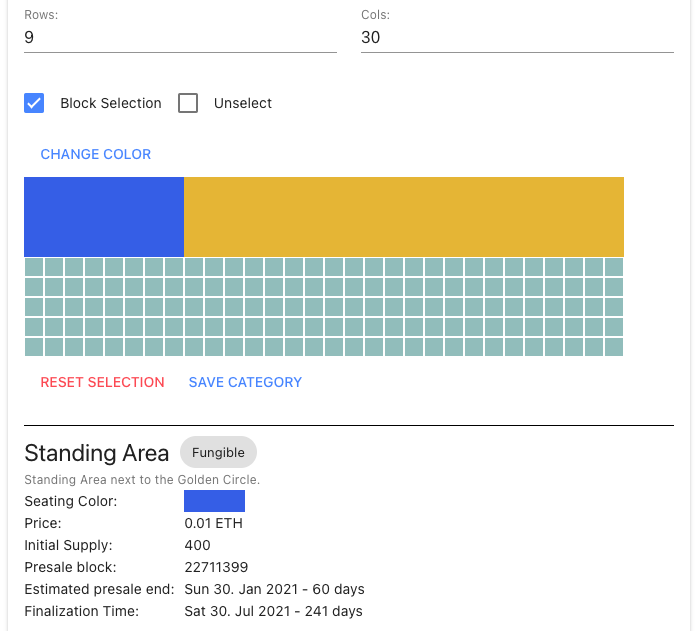
\includegraphics[width=14cm]{images/host-seating-plan.png}
    \caption{Seating plan \protect}
    \label{img:host-seating-plan}
\end{figure}

Currently, changes to the ticket metadata are allowed in our SCs. However, since in our design the seat mapping of a ticket type is also stored in the metadata, we do not provide such functionality in the host-client to prevent duplicated seats in the seating plan. This is addressed further as a potential future work task (see Section \ref{future-work-ticket-metadata-change}).

\subsection{ID Approver Registration and Identity Approval}
As extension to the host-client application, two views are included that support a basic interaction with the identity SC. The ID approver registration view contains a form to easily register as an ID approver with their supported methods, website and twitter. The website and twitter input fields also trigger a check for the trust certificates as in the event creation form. Once an ID approver is registered, the identity approval form allows to easily store the verification level of an account on the identity SC.

\section{Access Control}
% author: Nicolas Spielmann
The access control application is used to check, whether a guest is eligible to enter the event. To be eligible to enter, the guest needs to hold the right amount of the right type of tickets. This check needs to be done very fast, since a guest does not want to wait for the validity check when entering the venue and usually many guest should enter the venue within a short time frame. This could be tackled by doing the whole check of ticket ownership and invalidation off-chain. However, due to the implementation of the event SC, it is not trivial to obtain all current owner of a ticket and just save them to a database. Therefore, a hybrid approach was chosen.

This hybrid approach makes use of the fact, that once the Ethereum address is known, it is trivial to check for ticket ownership. The BC is only queried to obtain the amount of ticket the guest holds. Since this is a pure view transaction, this can be done very fast and does not cost anything. To make this query even faster, a local BC node could be run.

To ensure that guest can only enter once with the ticket, it is locally saved, how many tickets per Ethereum address entered to the event. When determine, whether a guest still has enough tickets, the local database and the BC are queried to calculate the number of remaining tickets. This also solves the problem of invalidation of tickets, since the ticket is considered as used, once it has been saved to the local database. An invalidation of tickets on-chain would have come with a very high cost, since all the tickets would require an Ethereum transaction to invalidate them, costing GAS payed by the event host.

%Author: Michael Bucher
\section{Access Terminal}\label{design:access-terminal}
The access terminal is the frontend component in the proposed access control solution in subsection \ref{subsection:access-control}. It is intended to be used on a tablet to display a QR code that contains the necessary information for the guest to validate the held tickets to enter the location.

The application is structured into two views. The connection view as shown in figure \ref{img:terminal-registration-form} contains a form to register the terminal with the set up backend. The required information is the base URL of the host backend, the secret that is stored in the backend to permit this device and the area where the guest is coming from and the area where the guest will be after passing the terminal. Currently there are five different areas provided, whereas the area \textit{entrance} must be used initially when a guest enters the location the first time. Finally, when the registration was successful, the application routes to the terminal view.

\begin{figure}[H]
    \centering
    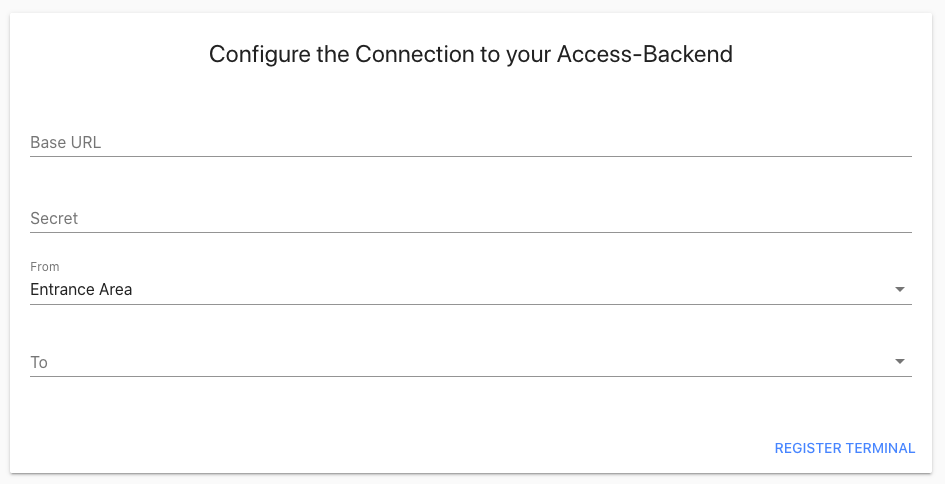
\includegraphics[width=15cm]{images/terminal-registration.png}
    \caption{Terminal Registration Form \protect}
    \label{img:terminal-registration-form}
\end{figure}

The terminal shows a QR code that contains a random message and the base URL of the backend. Whenever a guest requests the verification of its signature connected to this terminal the status changes to either \textit{granted} or \textit{denied}. Depending on that status a green or a red field is displayed on the terminal. Upon a click the terminal requests a new random message which also resets the status in the backend. This message is then displayed in a new QR code and the terminal awaits again a status change.


